\documentclass{sig-alternate}
\pagenumbering{arabic}

\usepackage[utf8]{inputenc}
\usepackage{amsmath}
\usepackage{amsfonts}
\usepackage{amssymb}
\usepackage{graphicx}
\usepackage[space]{grffile}
\graphicspath{figures/}
\usepackage{import}
\usepackage{url}
\usepackage{hyperref}

% http://tex.stackexchange.com/questions/57865/how-to-use-multiple-urls-for-one-bibtex-reference
\let\URL\url
\makeatletter
\def\url#1{\@URL#1||\@nil}
\def\@URL#1|#2|#3\@nil{%
  \URL{#1}\ifx\relax#2\relax\else| \URL{#2}\fi}
\makeatother

\usepackage{subcaption}
\usepackage{tikz}
\usepackage{siunitx}
\usepackage{todonotes}%[disable]
\let\OldTodo\todo
\renewcommand{\todo}{\OldTodo[inline]}
\newcommand{\todolater}[1]{}%{\todo{#1}}%
\RequirePackage[date=terse, isbn=true, doi=true, url=false, urldate=iso8601, maxbibnames=9, backref=false, backend=bibtex, style=ieee]{biblatex}
\addbibresource{securityupdates.bib}
\renewcommand{\bibfont}{\small}

\AtEveryBibitem{% Clean up the bibtex rather than editing it
 \clearname{editor} % remove editors
}

\newcommand{\daNumDataPoints}{153 Billion}
\newcommand{\daNumStartedApps}{122\,000}
\newcommand{\daNumInstalledApps}{175\,000}
\newcommand{\daNumVulnsUsed}{11}
\newcommand{\daSigNumDevices}{100}
\newcommand{\daSigNumDays}{100}
\newcommand{\daNumManufacturers}{261}
\newcommand{\daNumSigManufacturers}{9}
\newcommand{\daNumModels}{2\,380}
\newcommand{\daNumSigModels}{15}
\newcommand{\daOSVersionPercValidLines}{99.5\%}
\newcommand{\daOSTotalDaysData}{1\,140\,000}
\newcommand{\daMeanInsecurityPerc}{$87.3 \pm 0.0\%$}
\newcommand{\daMeanOutstandingVulnerabilities}{0.637}
\newcommand{\daUpdatedness}{$0.0558 \pm 0.0002$}
\newcommand{\daSecurityScore}{$2.75 \pm 0.00$}
\newcommand{\daNumFullVersions}{1\,140}
\newcommand{\daNumOSVersions}{45}
\newcommand{\daNumSigOSVersions}{23}
\newcommand{\daNumAPIVersions}{15}
\newcommand{\daNumFullVersionUpdates}{4\,220}
\newcommand{\daNumOSVersionUpdates}{3\,560}
\newcommand{\daNumFullOnlyVersionUpdates}{640}
\newcommand{\daNumSecurityUpdates}{1\,110}
\newcommand{\daNumPossibleSecurityUpdates}{2\,140}
\newcommand{\daTabSecScoresmanufacturer}{\begin{table} \centering \begin{tabular}{l|c|c|c|c} Name & $f$ & $u$ & $m$ & \textbf{Security score} \\ &&&& (out of 10) \\ \hline LG & $0.12 \pm 0.00$ & $0.32 \pm 0.00$ & 0.74 & $3.38 \pm 0.01$ \\  Motorola & $0.16 \pm 0.00$ & $0.13 \pm 0.00$ & 0.77 & $2.93 \pm 0.01$ \\  other & $0.13 \pm 0.00$ & $0.06 \pm 0.00$ & 0.64 & $2.75 \pm 0.00$ \\  Samsung & $0.14 \pm 0.00$ & $0.05 \pm 0.00$ & 0.71 & $2.67 \pm 0.00$ \\  Sony & $0.13 \pm 0.00$ & $0.18 \pm 0.00$ & 1.02 & $2.64 \pm 0.01$ \\  HTC & $0.14 \pm 0.00$ & $0.09 \pm 0.00$ & 0.89 & $2.55 \pm 0.00$ \\  asus & $0.15 \pm 0.00$ & $0.56 \pm 0.01$ & 6.06 & $2.30 \pm 0.02$ \\  Symphony & $0.00 \pm 0.00$ & $0.04 \pm 0.00$ & 4.79 & $0.19 \pm 0.00$ \\  walton & $0.00 \pm 0.00$ & $0.04 \pm 0.00$ & 5.79 & $0.14 \pm 0.01$ \\ \end{tabular} \caption{Security scores for manufacturers} \label{tab:sec_manufacturer} \end{table}}
\newcommand{\daTabSecScoresmodel}{\begin{table} \centering \begin{tabular}{l|c|c|c|c} Name & $f$ & $u$ & $m$ & \textbf{Security score} \\ &&&& (out of 10) \\ \hline Galaxy Nexus & $0.53 \pm 0.00$ & $0.53 \pm 0.01$ & 1.53 & $4.80 \pm 0.03$ \\  Nexus 4 & $0.23 \pm 0.00$ & $0.82 \pm 0.01$ & 6.06 & $3.39 \pm 0.04$ \\  Nexus 7 & $0.19 \pm 0.00$ & $0.74 \pm 0.01$ & 5.92 & $3.02 \pm 0.04$ \\  other & $0.13 \pm 0.00$ & $0.12 \pm 0.00$ & 0.64 & $2.94 \pm 0.00$ \\  Desire HD & $0.08 \pm 0.00$ & $0.05 \pm 0.00$ & 0.39 & $2.91 \pm 0.02$ \\  HTC Sensation & $0.36 \pm 0.00$ & $0.01 \pm 0.01$ & 1.59 & $2.47 \pm 0.02$ \\  GT-I9100 & $0.22 \pm 0.00$ & $0.02 \pm 0.00$ & 1.20 & $2.33 \pm 0.01$ \\  HTC Desire S & $0.02 \pm 0.00$ & $0.02 \pm 0.00$ & 1.00 & $1.75 \pm 0.01$ \\  GT-N7000 & $0.25 \pm 0.00$ & $0.00 \pm 0.00$ & 2.52 & $1.43 \pm 0.02$ \\  GT-P1000 & $0.01 \pm 0.00$ & $0.00 \pm 0.01$ & 1.73 & $0.94 \pm 0.02$ \\  GT-I9300 & $0.15 \pm 0.00$ & $0.01 \pm 0.00$ & 6.15 & $0.64 \pm 0.01$ \\  GT-I9505 & $0.00 \pm 0.00$ & $0.18 \pm 0.00$ & 6.77 & $0.55 \pm 0.01$ \\  GT-N7100 & $0.07 \pm 0.00$ & $0.00 \pm 0.01$ & 6.91 & $0.28 \pm 0.02$ \\  HTC Desire HD & $0.00 \pm 0.00$ & $0.00 \pm 0.01$ & 3.05 & $0.27 \pm 0.02$ \\ \end{tabular} \caption{Security scores for models} \label{tab:sec_model} \end{table}}
\newcommand{\daTabSecScoressummary}{\begin{table} \centering \begin{tabular}{l|c|c|c|c} Name & $f$ & $u$ & $m$ & \textbf{Security score} \\ &&&& (out of 10) \\ \hline nexus & $0.36 \pm 0.00$ & $0.51 \pm 0.00$ & 0.68 & $5.01 \pm 0.01$ \\  notnexus & $0.12 \pm 0.00$ & $0.04 \pm 0.00$ & 0.64 & $2.67 \pm 0.00$ \\ \end{tabular} \caption{Security scores for nexus} \label{tab:sec_summary} \end{table}}
\newcommand{\daUpdatednessPerc}{$5.58 \pm 0.02\%$}
\newcommand{\daNumOSDevices}{19\,000}
\newcommand{\daSigNumDevicesDay}{20}
\newcommand{\daSigNumDeviceDays}{10\,000}
\newcommand{\daTabAndVulns}{\begin{table} \centering \begin{tabular}{l|c|l} Vulnerability & Date known & How known \\ \hline KillingInTheNameOf psneuter ashmem & 2010-07-13 & Fixed on \\ exploid udev & 2010-07-15 & Discovered on \\ RageAgainstTheCage adb & 2010-08-21 & Discovered on \\ levitator & 2011-03-10 & Discovered on \\ Gingerbreak & 2011-04-18 & Fixed on \\ zergRush & 2011-10-06 & Discovered on \\ APK duplicate file & 2013-02-18 & Discovered on \\ APK unchecked name & 2013-06-30 & Discovered on \\ APK unsigned shorts & 2013-07-03 & Fixed on \\ keystore buffer & 2013-09-09 & Discovered on \\ TwerkMyMoto & 2013-11-24 & Discovered on \\ vold asec & 2014-01-27 & Fixed on \\\end{tabular} \caption{Root equivalent vulnerabilities in Android} \label{tab:andvulns} \end{table}}
\newcommand{\daOSYearsOfData}{3}
\newcommand{\daSecScoreBestmanufacturer}{LG}
\newcommand{\daSecScoreWorstmanufacturer}{walton}
\newcommand{\daSecScoreBestmodel}{Galaxy Nexus}
\newcommand{\daSecScoreWorstmodel}{HTC Desire HD A9191}
\newcommand{\daSecScoreBestsummary}{nexus}
\newcommand{\daSecScoreWorstsummary}{notnexus}
\newcommand{\daSecScoreBestmanufacturerScore}{$3.38 \pm 0.01$}
\newcommand{\daSecScoreWorstmanufacturerScore}{$0.139 \pm 0.006$}
\newcommand{\daSecScoreBestmodelScore}{$4.8 \pm 0.0$}
\newcommand{\daSecScoreWorstmodelScore}{$0.274 \pm 0.020$}
\newcommand{\daSecScoreBestsummaryScore}{$4.1 \pm 0.0$}
\newcommand{\daSecScoreWorstsummaryScore}{$2.9 \pm 0.0$}
\newcommand{\daVulnFree}{$0.127 \pm 0.000$}
\newcommand{\daAdbEnabledPerc}{$19.5 \pm 0.0\%$}
\newcommand{\daNumUpdatesUpgrades}{3\,330}
\newcommand{\daNumUpdatesDowngrades}{147}
\newcommand{\daPercUpdatesDowngrades}{$3.58 \pm 0.3\%$}
\newcommand{\daStartDate}{2011-07-01}
\newcommand{\daEndDate}{2014-11-07}
\newcommand{\daNumOperators}{1\,390}
\newcommand{\daTabSecScoresoperator}{\begin{table} \centering \begin{tabular}{l|c|c|c|c} Name & $f$ & $u$ & $m$ & \textbf{Security score} \\ &&&& (out of 10) \\ \hline O2 uk & $0.25 \pm 0.00$ & $0.12 \pm 0.00$ & 0.37 & $3.79 \pm 0.01$ \\  T-Mobile & $0.19 \pm 0.00$ & $0.18 \pm 0.00$ & 0.48 & $3.57 \pm 0.01$ \\  Orange & $0.21 \pm 0.00$ & $0.09 \pm 0.00$ & 0.39 & $3.52 \pm 0.02$ \\  Sprint & $0.18 \pm 0.00$ & $0.11 \pm 0.00$ & 0.44 & $3.41 \pm 0.01$ \\  3 & $0.15 \pm 0.00$ & $0.09 \pm 0.00$ & 0.49 & $3.15 \pm 0.01$ \\  AT\&T & $0.12 \pm 0.00$ & $0.08 \pm 0.00$ & 0.43 & $3.08 \pm 0.01$ \\  Vodafone uk & $0.13 \pm 0.00$ & $0.10 \pm 0.00$ & 0.52 & $3.07 \pm 0.01$ \\  Verizon & $0.18 \pm 0.00$ & $0.09 \pm 0.00$ & 0.81 & $2.82 \pm 0.01$ \\  unknown & $0.10 \pm 0.00$ & $0.22 \pm 0.00$ & 1.08 & $2.57 \pm 0.01$ \\  n Telenor & $0.03 \pm 0.00$ & $0.10 \pm 0.00$ & 1.42 & $1.59 \pm 0.01$ \\  Airtel & $0.06 \pm 0.00$ & $0.03 \pm 0.00$ & 1.93 & $1.10 \pm 0.01$ \\  Grameenphone & $0.01 \pm 0.00$ & $0.02 \pm 0.00$ & 1.99 & $0.80 \pm 0.00$ \\  Robi & $0.00 \pm 0.00$ & $0.04 \pm 0.00$ & 2.19 & $0.73 \pm 0.01$ \\  banglalink & $0.00 \pm 0.00$ & $0.03 \pm 0.00$ & 2.90 & $0.40 \pm 0.00$ \\ \end{tabular} \caption{Security scores for operators} \label{tab:sec_operator} \end{table}}
\newcommand{\daSecScoreBestoperator}{O2 uk}
\newcommand{\daSecScoreBestoperatorScore}{$3.79 \pm 0.01$}
\newcommand{\daSecScoreWorstoperator}{banglalink}
\newcommand{\daSecScoreWorstoperatorScore}{$0.4 \pm 0.0$}
\newcommand{\daNumSigOperators}{14}
\newcommand{\daMonthsDevices}{1\,600}
\newcommand{\daMonths}{6}
\newcommand{\daSigVersionPerc}{1\%}
\newcommand{\daSigVersionDays}{10}
\newcommand{\daNumDeviceDataDevices}{50}
\newcommand{\daNumSigFullVersions}{83}
\newcommand{\daSecScoreBestmanufacturerNumFullVersions}{104}
\newcommand{\daSecScoreworstmanufacturerNumFullVersions}{239}
\newcommand{\daSecScoreBestmodelNumFullVersions}{49}
\newcommand{\daSecScoreworstmodelNumFullVersions}{2}
\newcommand{\daSecScoreBestsummaryNumFullVersions}{73}
\newcommand{\daSecScoreworstsummaryNumFullVersions}{1057}
\newcommand{\daSecScoreBestoperatorNumFullVersions}{88}
\newcommand{\daSecScoreworstoperatorNumFullVersions}{89}
\newcommand{\daSecScoreWorstmanufacturerNumFullVersions}{20}
\newcommand{\daSecScoreWorstmodelNumFullVersions}{2}
\newcommand{\daSecScoreWorstsummaryNumFullVersions}{1103}
\newcommand{\daSecScoreWorstoperatorNumFullVersions}{59}
\newcommand{\daFullDeployedAt}{95\%}
\newcommand{\daOSCurveFitParamFirst}{87.5}
\newcommand{\daOSCurveFitParamSecond}{\num{0.00315}}
\newcommand{\daOSCurveFitRMSE}{0.114}
\newcommand{\daAPICurveFitParamFirst}{110}
\newcommand{\daAPICurveFitParamSecond}{\num{0.00315}}
\newcommand{\daAPICurveFitRMSE}{0.116}
\newcommand{\daOSCurvePolyRMSE}{0.115}
\newcommand{\daOSCurveSplineRMSE}{0.115}
\newcommand{\daOSCurveHalfDeployed}{$308 \pm 81$}
\newcommand{\daOSCurveFullDeployed}{$1\,040 \pm 236\,000$}
\newcommand{\daAPICurvePolyRMSE}{0.117}
\newcommand{\daAPICurveSplineRMSE}{0.117}
\newcommand{\daAPICurveHalfDeployed}{$330 \pm 84$}
\newcommand{\daAPICurveFullDeployed}{$1\,060 \pm 236\,000$}
\newcommand{\daVulnAPKDuplicateFileOctoberPerc}{91.5\%}
\newcommand{\daNumUpdatesBigUpgrades}{778}
\newcommand{\daNumUpdatesSkippedBig}{3}
\newcommand{\daPercBigUpgrades}{$18.9 \pm 0.7\%$}
\newcommand{\daUpdatesPerYear}{$1.35 \pm 0.02$}
\newcommand{\daOSMonthsOfData}{40}
\newcommand{\daMeanInsecurityPercNominal}{87.3\%}
\newcommand{\daVulnFreeNominal}{0.127}
\newcommand{\daUpdatednessNominal}{0.0558}
\newcommand{\daUpdatednessPercNominal}{5.58\%}
\newcommand{\daSecurityScoreNominal}{2.75}
\newcommand{\daUpdatesPerYearNominal}{1.35}
\newcommand{\daOSCurveHalfDeployedNominal}{308}
\newcommand{\daOSCurveFullDeployedNominal}{1\,040}
\newcommand{\daAPICurveHalfDeployedNominal}{330}
\newcommand{\daAPICurveFullDeployedNominal}{1\,060}
\newcommand{\daSecScoreBestoperatorScoreNominal}{3.79}
\newcommand{\daSecScoreWorstoperatorScoreNominal}{0.4}
\newcommand{\daSecScoreBestmodelScoreNominal}{4.8}
\newcommand{\daSecScoreWorstmodelScoreNominal}{0.274}
\newcommand{\daAdbEnabledPercNominal}{19.5\%}
\newcommand{\daSecScoreBestmanufacturerScoreNominal}{3.38}
\newcommand{\daSecScoreWorstmanufacturerScoreNominal}{0.139}
\newcommand{\daUpdatesPerMonthPerVersion}{$3.62 \pm 0.06$}
\newcommand{\daNumUpdateFullOnly}{637}
\newcommand{\daVulnZergRushMonthsDefFixDeployed}{27.3}
\newcommand{\daUpdatesPerMonthPerVersionNominal}{3.62}
\newcommand{\daPercBigUpgradesNominal}{18.9\%}
\newcommand{\daPercUpdatesDowngradesNominal}{3.58\%}

\newcommand{\da}{Device Analyzer}
\newcommand{\dafoot}{\textsuperscript{\ref{foot:dadata}}}
\newcommand{\avoNumSubmitters}{7}
\newcommand{\avoTotalExternalLines}{25 Million}
\newcommand{\avoNumExternalProjects}{176}
\newcommand{\avoNumBigExternalLinesOfCode}{25 Million}
\newcommand{\avoBigExternalLinesOfCodePerc}{99.7\%}
\newcommand{\avoNumVulnerabilities}{32}
\newcommand{\avoNumVulnAllAndroid}{15}
\newcommand{\avoNumVulnSpecific}{17}
\newcommand{\avoStartDate}{2013-08-28}
\newcommand{\avoEndDate}{2015-03-24}
\newcommand{\avoFirstDataDateMonth}{July 2010}
\newcommand{\avoFirstDataDate}{2010-07-13}
\newcommand{\avoLastDataDateMonth}{March 2015}
\newcommand{\avoLastDataDate}{2015-03-12}
\newcommand{\avoVulnsPerYearNominal}{6.86}
\newcommand{\avoVulnsPerYear}{$6.86 \pm 1.21$}
\newcommand{\avoVulnsPerYearAllAndroidNominal}{3.21}
\newcommand{\avoVulnsPerYearAllAndroid}{$3.21 \pm 0.83$}
\newcommand{\avoVulnsPerYearTwosfNominal}{6.9}
\newcommand{\avoVulnsPerYearTwosf}{$6.9 \pm 1.2$}
\newcommand{\avoVulnsPerYearAllAndroidTwosfNominal}{3.2}
\newcommand{\avoVulnsPerYearAllAndroidTwosf}{$3.2 \pm 0.0$}
\newcommand{\avoTabAndVulns}{\begin{table} \centering \small \begin{tabular}{l|l|c|c} Vulnerability & How known & Date & Categories\\ \hline KillingInTheNameOf & Fixed on & 2010-07-13 & system, kernel\\ exploid udev & Discovered on & 2010-07-15 & kernel\\ levitator & Discovered on & 2011-03-10 & kernel\\ Gingerbreak & Fixed on & 2011-04-18 & system\\ zergRush & Discovered on & 2011-10-06 & system\\ APK duplicate file & Discovered on & 2013-02-18 & signature\\ APK unchecked name & Discovered on & 2013-06-30 & signature\\ APK unsigned shorts & Fixed on & 2013-07-03 & signature\\ vold asec & Fixed on & 2014-01-27 & system\\ Fake ID & Fixed on & 2014-04-17 & signature\\ TowelRoot & Discovered on & 2014-05-03 & kernel\\\end{tabular} \caption{Critical vulnerabilities in Android} \label{tab:andvulns} \end{table}}
\newcommand{\avoNumBigExternalProjects}{40}
\newcommand{\avoNumAnalysedExternalProjects}{28}
\newcommand{\avoNumAnalysedExternalLinesOfCode}{6 Million}
\newcommand{\avoAnalysedExternalLinesOfCodePerc}{24.9\%}
\newcommand{\avoBigExternalMedianVersions}{2.0}
\newcommand{\avoBigExternalMeanVersionsNominal}{2.57}
\newcommand{\avoBigExternalMeanVersions}{$2.57 \pm 1.84$}
\newcommand{\avoBigExternalTotalVersions}{72}

\newcommand{\avo}{AVO}
\newcommand{\percMarketShare}{83.6\%~\footnote{\url{http://www.theinquirer.net/inquirer/news/2379036/android-hits-836-percent-marketshare-while-ios-windows-and-blackberry-slide}}}
\newcommand{\daNumDevices}{\daNumOSDevices}
\newcommand{\daDeviceDays}{\daOSTotalDaysData}
% Num versions since \daStartDate
\newcommand{\opensslNumVersions}{59}
\newcommand{\linuxNumVersions}{618}
\newcommand{\linuxMeanUpdateLatency}{$137 \pm 48$}
\newcommand{\opensslMeanUpdateLatency}{$120 \pm 55$}
\newcommand{\bouncycastleNumVersions}{6}
\newcommand{\bouncycastleMeanUpdateLatency}{$239 \pm 78$}
\newcommand{\linuxMeanUpdateLatencyNominal}{137}
\newcommand{\opensslMeanUpdateLatencyNominal}{120}
\newcommand{\bouncycastleMeanUpdateLatencyNominal}{239}

\newcommand{\otherProjNum}{\avoNumExternalProjects}%TODO check we are doing the right calculation here and not overcounting

% Blinding function
\newcommand{\identifying}[1]{#1}%{}%
\newcommand{\blindauthors}[1]{#1}%{Paper \#XX}%

% Terminology

% Android, Unix, adb
% update, release, patch: what do we actually mean and what relevance does that have to security?
% Device manufacturers
% Network operators
% Device model TODO check
% Device handset TODO check


\begin{document}
%
% --- Author Metadata here ---
\conferenceinfo{SPSM}{2015 Denver, Colorado, USA}
%\CopyrightYear{2015} % Allows default copyright year (20XX) to be over-ridden - IF NEED BE.
%\crdata{0-12345-67-8/90/01}  % Allows default copyright data (0-89791-88-6/97/05) to be over-ridden - IF NEED BE.
% --- End of Author Metadata ---

\title{Measuring security performance in the Android ecosystem}

\numberofauthors{3}
\author{
\href{http://orcid.org/0000-0001-8936-0683}{Daniel~R.~Thomas}
\and
Alastair~R.~Beresford\\
       \affaddr{Computer Laboratory}\\
       \affaddr{University of Cambridge}\\
       \affaddr{Cambridge, United Kingdom}\\
       \email{Firstname.Lastname@cl.cam.ac.uk}
\and
Andrew~Rice
}


\maketitle

\begin{abstract}
The security of Android is severely damaged by the lack of security updates for known critical vulnerabilities  being shipped to devices.
We find there is significant variability in the timely delivery of security updates across different device manufacturers and mobile network operators, and we define a security metric to rank the performance of device manufacturers and network operators in our data set.
This provides the comparable data required for purchasers to determine which device manufacturers and network operators to use and hence incentives them to ship security updates.
\end{abstract}

% A category with the (minimum) three required fields
\category{Security and privacy}{Systems security}{Operating systems security}[Mobile platform security]
\category{Security and privacy}{Systems security}{Vulnerability management}

\terms{Economics, Measurement, Security}

\keywords{Android, updates, vulnerabilities, metrics, ecosystems}

\section{Introduction}

We have found that Android devices do not receive security updates promptly when critical vulnerabilities are publicly disclosed and hence \daMeanInsecurityPercNominal\ are exposed to known critical vulnerabilities~\cite{androidvulnerabilities.org}.
Here we attempt to determine why by understanding the Android update process, apportioning blame to different entities in the ecosystem and producing a scoring metric to compare different entities.

By producing a scoring metric which compares different entities such as device manufacturers, network operators or specific device models we can provide information which allows device purchasers to select devices with better security.
Currently corporate and public sector buyers are encouraged to purchase secure devices, but we have found little concrete guidance on the specific makes and models providing the best security.
For example, CESG, which advises the UK government on how to secure its computer systems, recommends picking Android device models from device manufactures which are good at shipping security updates promptly but it does not state which device manufacturers these are~\cite{CESG2013}.
We are also collaborating with a FTSE 100 company to give them concrete information to answer this question.
To address this, we developed a scoring system and provide numbers on the historic performance of device models in the \da\ project in~\S\ref{sec:security_scoring}.
We provide the answer to the question ``Who should I buy my Android phone from for best security?'', in general Nexus devices are better, further details are given in \S\ref{sec:security_scoring:results}.

The Android update process is slow because its development is distributed among many parties and has a long multi-stage pipeline~\cite{HTC2013}.
The security of Android relies on many open source projects, include the Linux kernel, OpenSSL and BouncyCastle as well as Google who build the core platform.
In addition, device manufacturers (we know of \daNumManufacturers\footnote{\label{foot:dadata}We computed this from the \da~\cite{Wagner2013} data, see \S\ref{sec:android_update_process}.}) and network operators (\daNumOperators\dafoot) may make further modifications before devices are shipped to customers.
Understanding this ecosystem is important as device manufacturers have introduced additional vulnerabilities in the past~\cite{Grace2012}.
We present a better understanding of both the ecosystem of Android development and associated vulnerabilities more fully in \S\ref{sec:android_ecosystem}.

\begin{figure}
\centering
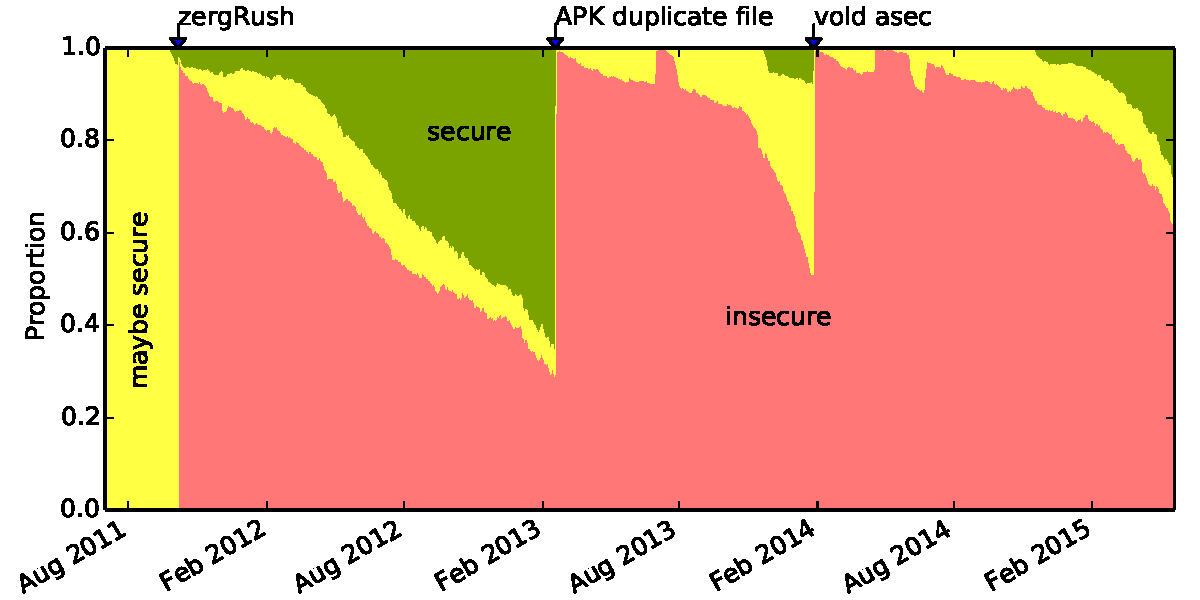
\includegraphics[width=\columnwidth]{figures/proportioninsecure}
\caption{Proportion of devices running insecure, maybe secure and secure versions of Android against time.
The red vertical lines are caused by vulnerabilities being discovered with those which have the biggest impact annotated.
}
\label{fig:proportioninsecure}
\end{figure}
By using data from \da~\cite{Wagner2013} we can examine the versions of Android running on user devices over time and through comparison with data on which versions of Android were vulnerable to different critical vulnerabilities~\cite{androidvulnerabilities.org} we can plot the exposure of Android devices to known critical vulnerabilities.
Figure~\ref{fig:proportioninsecure} shows that Android devices are often exposed to known security vulnerabilities.
One solution to this problem is regulation, and indeed there is ongoing legal action to force network operators to ship updates for security vulnerabilities~\cite{Soghoian2013}.\todolater{Check on the status of this legal action}
Many smartphones are sold on 12--24 month contracts, and yet our data shows many devices do not receive many security updates, with an overall average of \daUpdatesPerYearNominal\ per year. 
In contrast, Windows XP could be purchased for a one-off payment in October 2001 and received security updates monthly until April 2014.
An alternative to regulation is access to publicly available data.
Comparative data, which we provide in this paper, would provide an incentive to both device manufacturers and network operators to provide updates.

In summary, the contributions of this paper are:
\begin{itemize}
 \item We quantify the Android update process~\S\ref{sec:android_ecosystem}.
 \item We propose the FUM scoring metric to evaluate the security of different instances of a platform~\S\ref{sec:security_scoring:method}.
 \item We measure the security of Android according to this and compare different device manufacturers, device models and network operators to allow device purchasers to differentiate between them based on security~\S\ref{sec:security_scoring:results}.
\end{itemize}


\section{Android Ecosystem}\label{sec:android_ecosystem}
There is a complex Android ecosystem which creates and distributes updates to Android which fix vulnerabilities.
In this section we describe how the Android ecosystem functions and how Android versions are produced, as seen by the \da\ project.


\subsection{Android update process}

\label{sec:android_update_process}
\begin{figure}[h]
 \centering
 \def\svgwidth{\columnwidth}
 \import{figures/}{update_ecosystem.pdf_tex}
 \caption{Flow of updates between participants in the Android ecosystem.
 Numbers on edges indicate updates shipped between \daStartDate\ and \daEndDate, those in brackets represent number of such entities.
 Dotted arrows indicate flows where we can't measure how many updates are produced as they are not public.}
 \label{fig:update_ecosystem}
\end{figure}
To understand how vulnerabilities in Android are fixed we examine the Android update process which we model in Figure~\ref{fig:update_ecosystem}.
There are five entities or groups which contribute towards Android updates: the network operators, the device manufacturers, the hardware developers, Google and the upstream open source projects.
Android builds on various open source projects such as the Linux kernel, OpenSSL and BouncyCastle cryptography libraries.
Consequently Android can include any compatible versions of those projects, including those which fix security vulnerabilities.
Android also incorporates various drivers for different bits of hardware.
The Android platform is then built from these components by Google.
The code for each Android release or update is kept secret until after a binary release has been published.\footnote{\url{https://source.android.com/source/code-lines.html}}
Device manufacturers likely receive advanced access in order to prepare handsets so they can customise it before passing it on to the network operator.
The network operator may then make or request further customisations and perform further testing before shipping the update to the Device.
Sometimes device manufactures ship updates directly to the user, sometimes the device manufacturer and Google collaborate closely to make a particular phone, such as with Nexus devices.
Sometimes device manufacturers incorporate upstream open source project releases directly, and sometimes incorrectly -- for example previous work has recorded evidence of broken nightly builds of sqlite in Android releases~\cite{Wagner2013}.

The numbers of devices (\daNumOSDevices), network operators (\daNumOperators) and device manufacturers (\daNumManufacturers) in Figure~\ref{fig:update_ecosystem} come from the \da\ data.
Device manufacturer and network operator counts were obtained by normalising the results reported by Android to \da\ of the device manufacturer and active network operator.
This normalisation is a manual task involves removing invalid values (such as `manufacturer' or `airplane mode is on'), collating across company name changes (e.g.\ `lge' to `LG'), normalising punctuation, removing extra strings sometimes added such as (`(2g)' or `communications') and mapping some incorrectly placed model names back to their manufacturer.
This normalisation is not perfect and so these are overestimates on the \da\ data but they are likely still underestimates as there will be some device manufacturers and network operators which are not included in the \da\ data.

In Figure~\ref{fig:update_ecosystem} the number of updates received by devices (\daNumFullVersions) is the number of different full version strings observed in \da.
The number of updates shipped by Google (\daNumSigOSVersions) is the number of Android versions reported in \da\ which affected more than \daSigVersionPerc\ of devices for more than \daSigVersionDays\ days.
This significance test is to remove spurious versions recorded in \da\ such as `5.2.0' in 2012 which had still not been released in 2014.

We extracted data on the external projects used in Android and have included this and the scripts which generated it in AndroidVulnerabilities.org (\avo)~\cite{androidvulnerabilities.org}.
These scripts analysed the Android Open Source Project's source tree to examine the source code of each of the external projects to find the project version associated with each Android version tag on the repository.
There are \avoNumExternalProjects\ external open source projects in Android, contributing \avoTotalExternalLines\ lines of code.\footnote{Lines of code were measured using David A. Wheeler's \texttt{sloccount}.}
We analysed the top \avoNumBigExternalProjects\ by lines of code (\avoBigExternalLinesOfCodePerc\ of the total) and were able to automatically extract the versions of those projects included in different versions of Android for \avoNumAnalysedExternalProjects\ of these (\avoAnalysedExternalLinesOfCodePerc\ of the total).
We found \avoBigExternalTotalVersions\ distinct versions, a median of \avoBigExternalMedianVersions\ and mean of \avoBigExternalMeanVersions\ versions per project.
Android rarely changes the version of external projects it includes.

%An analysis by Vidas et al.~\cite{Vidas2011} of the Android 2.1 to 2.2 update found that it took 11 months from when Google released 2.2 for the last device which they were investigating to get the update.
To compute the latency between upstream releases and their inclusion in Android we scraped the release pages for those projects, to obtain the version numbers and release dates.
This allows us to compute the latency between an upstream project being released and it being included in Android, this is shown in Table~\ref{tab:update_ecosystem}.
The versions included in Android were about half a year old when the first version of Android containing it was released.
\begin{table}
\centering
\normalsize
\begin{tabular}{l|r|r}
Project	&	\# releases	&	latency (days) \\ \hline
linux	&	\linuxNumVersions	&	\linuxMeanUpdateLatency \\
openssl	&	\opensslNumVersions	&	\opensslMeanUpdateLatency \\
bouncycastle	&	\bouncycastleNumVersions	&	\bouncycastleMeanUpdateLatency \\
\end{tabular}
\caption{Flow of updates from upstream projects into Android. Number of updates as in Figure~\ref{fig:update_ecosystem}, latency in days for all pairs of versions we have data on.\todolater{scrape the other 26 websites... is it worth it?}}
\label{tab:update_ecosystem}
\end{table}

\todo{Do we want to talk about more stuff from the Esorics submission?}

\section{Comparing device manufacturers, device models and network operators}
\label{sec:security_scoring}\label{sec:exp:security_score}

To allow buyers of Android devices to purchase those devices which have the best security they need to know how different device manufacturers, device models and network operators compare in terms of the security they provide.
We propose a method to score a device manufacturer, device model or network operator based on its historic performance at keeping devices up-to-date and fixing security vulnerabilities.
We find that Android as a whole gets a score of \daSecurityScore\ out of 10, the highest scoring device manufacturer is \emph{\daSecScoreBestmanufacturer} (\daSecScoreBestmanufacturerScore\ out of 10) and the lowest scoring is \emph{\daSecScoreWorstmanufacturer} (\daSecScoreWorstmanufacturerScore\ out of 10).

\subsection{Method: Scoring for security}\label{sec:security_scoring:method}

Computing how good a particular device manufacturer or device model is from a security standpoint is difficult as it depends on a number of factors which are hard to observe, particularly on a large scale.
Ideally we would consider both the prevalence of potential problems which were not exploited and actual security failures.
%\footnote{A perfectly secure operating system would among other things detect and prevent all phishing attacks, provide perfect principle of least privilege isolation, not have any vulnerabilities, instantly fix all discovered vulnerabilities, not allow any user data to be used in a way which the user does not approve of and be really easy for an ordinary person to use.}
However in the absence of such data we propose a scheme for assigning a device a score out of ten based on data which can be observed, is based on previous metrics, and which we expect correlates with the actual security of the devices.

The FUM score is computed from three components:
\begin{description}
  \item[free $f$] The proportion of running devices which were free from critical vulnerabilities over time. This is equivalent to Acer and Jackson's proposal to measure the security based on the proportion of users with at least one unpatched critical vulnerability~\cite{Acer2010} and similar to the Vulnerability Free Days (VFD) score~\cite{Wright2014}.
  Unlike VFD this is the proportion of running devices which were free from critical vulnerabilities over time, rather than days which the device manufacturer was free from outstanding critical vulnerabilities as that does not take account of the update process.
  \item[update $u$] The proportion of devices which run the latest version of Android shipped to any device produced by that device manufacturer. This is a measure of internal updatedness, a low score would mean many devices are being left behind.
  This assumes that newer versions are better with stronger security.
  Historically steps have been taken to improve Android security in newer versions so this assumption should generally hold, but sometimes new updates introduce new vulnerabilities.
  \item[mean $m$] The mean number of outstanding vulnerabilities affecting devices not fixed on any device shipped by the device manufacturer. This is related to the Median Active Vulnerabilities (MAV) measure~\cite{Wright2014} but is the mean rather than the median, as this gives a continuous value.
  An example is given in Figure~\ref{fig:mcalculation}.
%TODO should we compute the median instead?
\end{description}

\begin{figure}
\centering
%\includegraphics[width=\columnwidth]{figures/mcalculation}
% Graphic for TeX using PGF
% Title: /home/drt24/git/papers/da/securityupdates/figures/mcalculation.dia
% Creator: Dia v0.97.3
% CreationDate: Wed Apr 22 15:03:07 2015
% For: drt24
% \usepackage{tikz}
% The following commands are not supported in PSTricks at present
% We define them conditionally, so when they are implemented,
% this pgf file will use them.
\ifx\du\undefined
  \newlength{\du}
\fi
\setlength{\du}{5\unitlength}
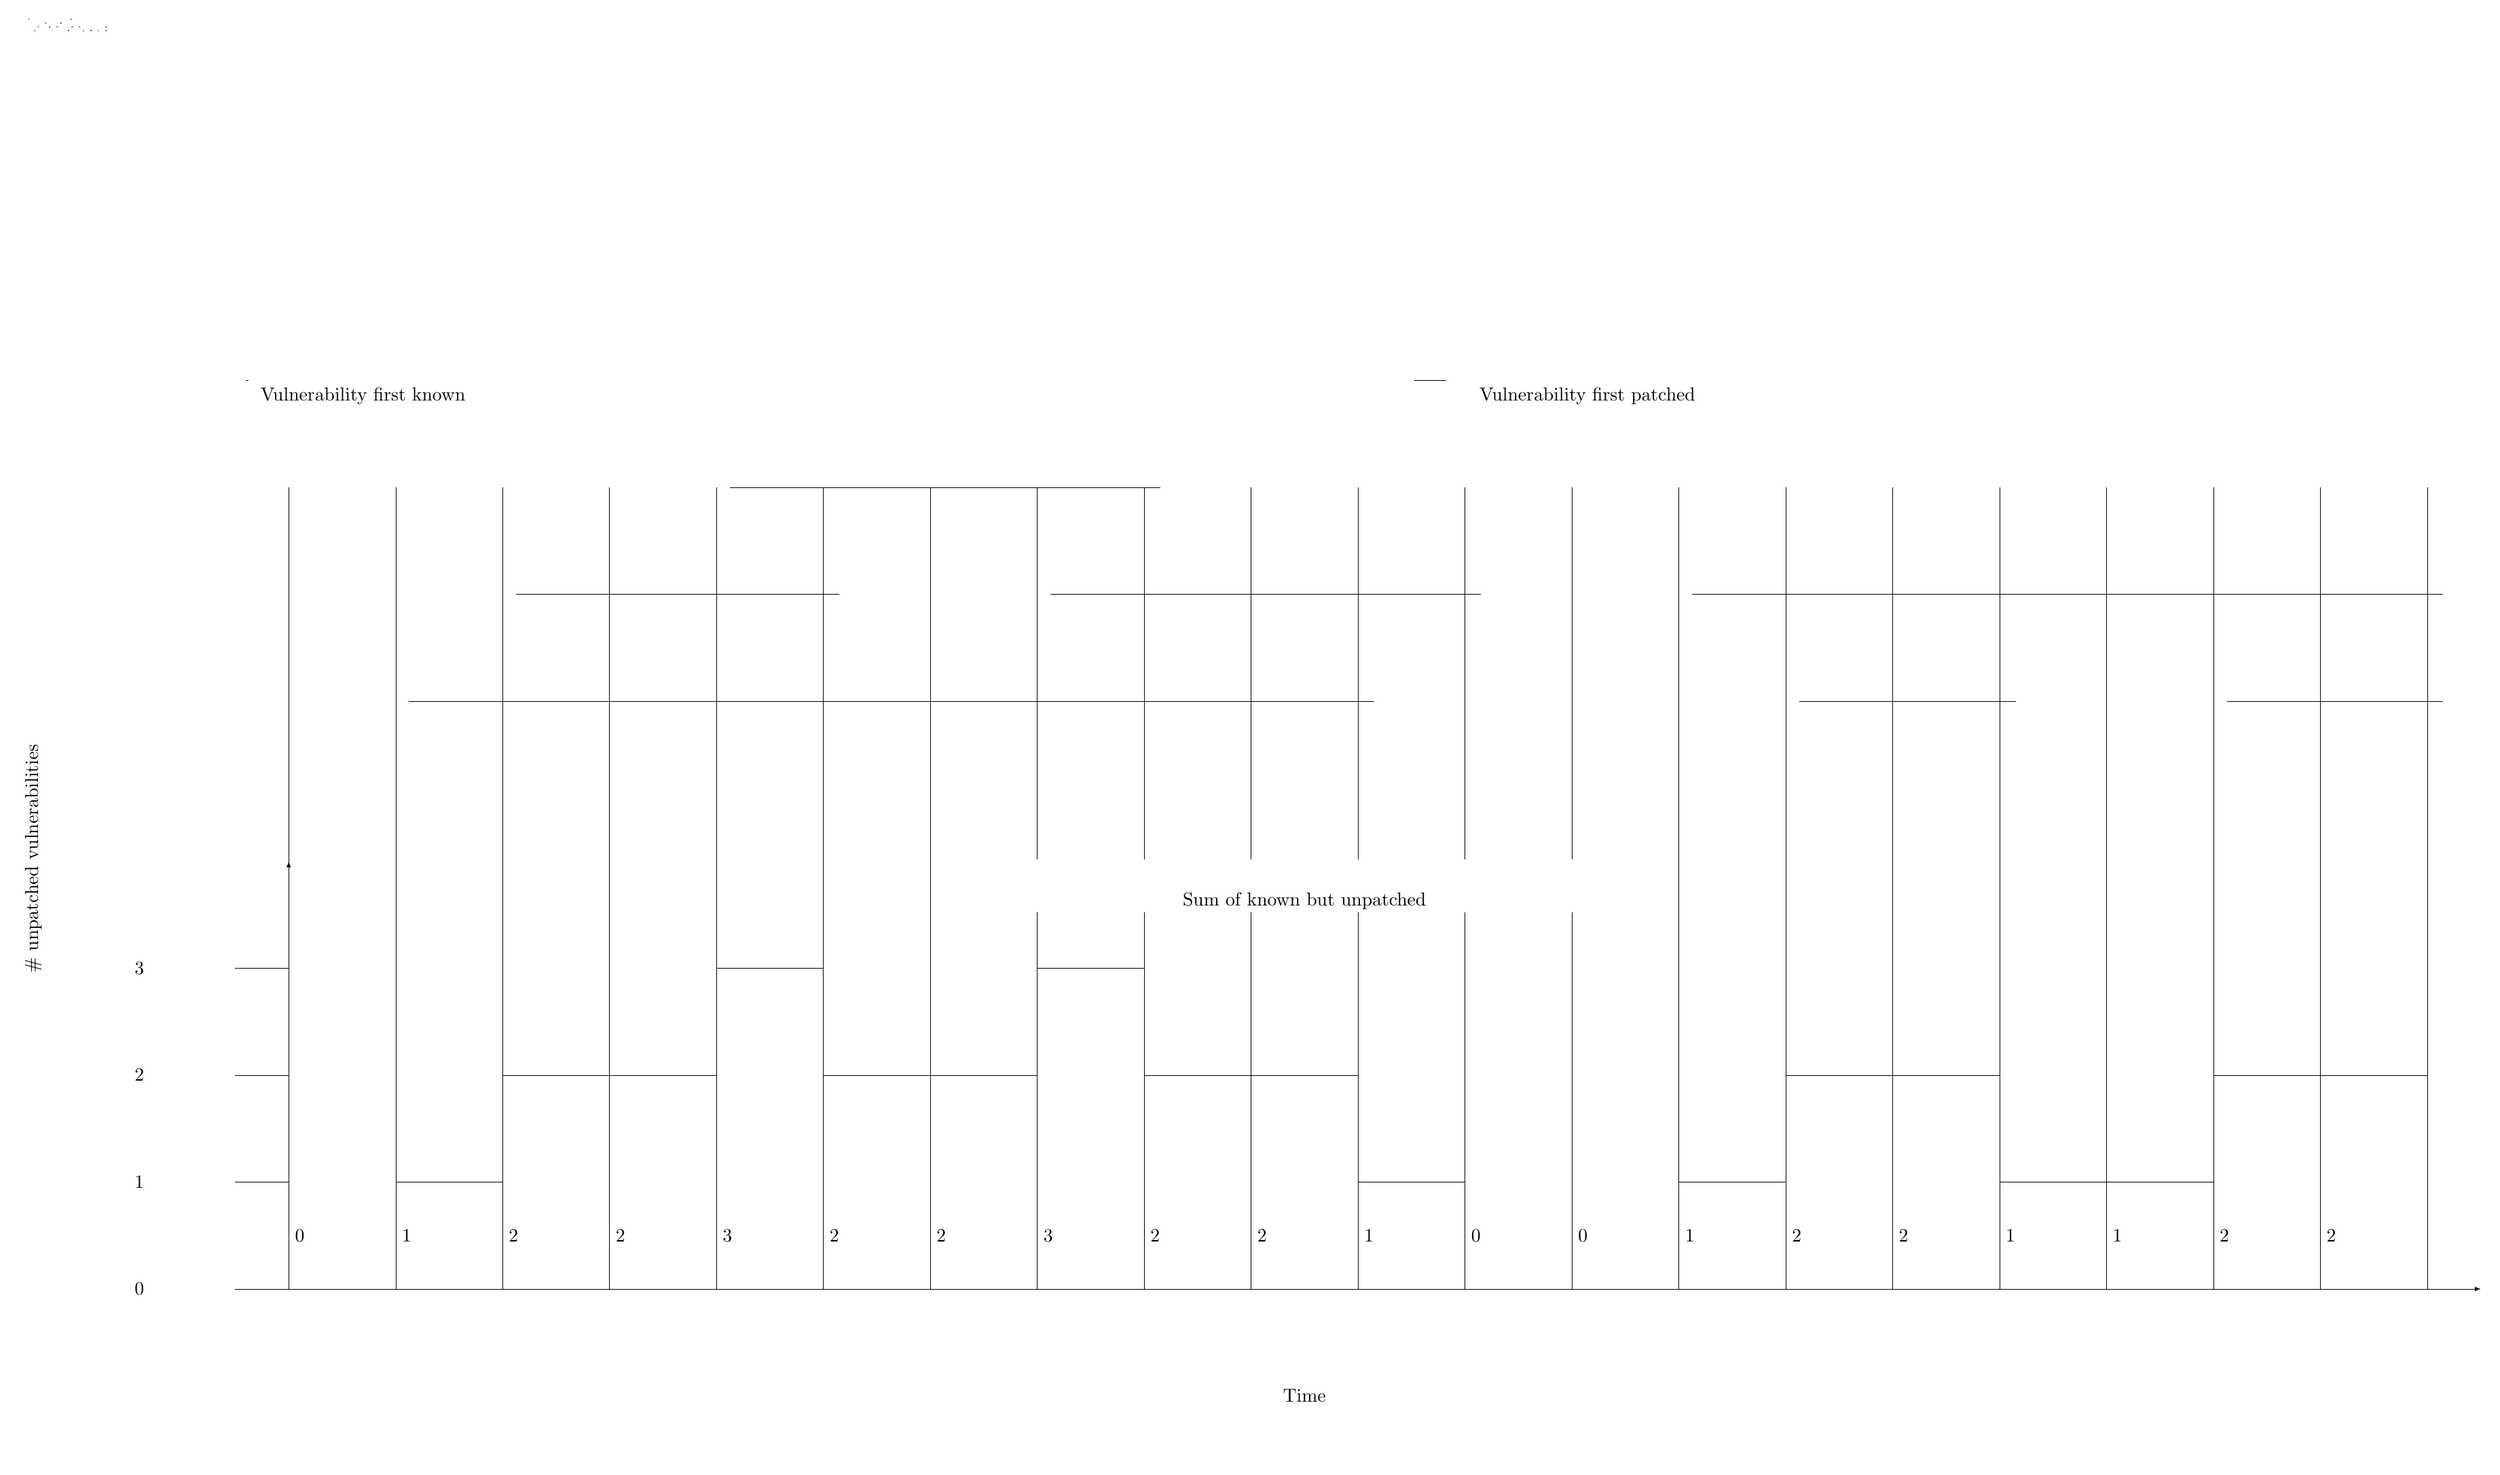
\begin{tikzpicture}
\pgftransformxscale{1.000000}
\pgftransformyscale{-1.000000}
\definecolor{dialinecolor}{rgb}{0.000000, 0.000000, 0.000000}
\pgfsetstrokecolor{dialinecolor}
\definecolor{dialinecolor}{rgb}{1.000000, 1.000000, 1.000000}
\pgfsetfillcolor{dialinecolor}
\pgfsetlinewidth{0.100000\du}
\pgfsetdash{{\pgflinewidth}{0.200000\du}}{0cm}
\pgfsetdash{{\pgflinewidth}{0.200000\du}}{0cm}
\pgfsetbuttcap
{
\definecolor{dialinecolor}{rgb}{0.000000, 0.000000, 0.000000}
\pgfsetfillcolor{dialinecolor}
% was here!!!
\definecolor{dialinecolor}{rgb}{0.000000, 0.000000, 0.000000}
\pgfsetstrokecolor{dialinecolor}
\draw (5.000000\du,24.000000\du)--(5.000000\du,9.000000\du);
}
\pgfsetlinewidth{0.100000\du}
\pgfsetdash{{\pgflinewidth}{0.200000\du}}{0cm}
\pgfsetdash{{\pgflinewidth}{0.200000\du}}{0cm}
\pgfsetbuttcap
{
\definecolor{dialinecolor}{rgb}{0.000000, 0.000000, 0.000000}
\pgfsetfillcolor{dialinecolor}
% was here!!!
\definecolor{dialinecolor}{rgb}{0.000000, 0.000000, 0.000000}
\pgfsetstrokecolor{dialinecolor}
\draw (7.000000\du,24.000000\du)--(7.000000\du,9.000000\du);
}
\pgfsetlinewidth{0.100000\du}
\pgfsetdash{{\pgflinewidth}{0.200000\du}}{0cm}
\pgfsetdash{{\pgflinewidth}{0.200000\du}}{0cm}
\pgfsetbuttcap
{
\definecolor{dialinecolor}{rgb}{0.000000, 0.000000, 0.000000}
\pgfsetfillcolor{dialinecolor}
% was here!!!
\definecolor{dialinecolor}{rgb}{0.000000, 0.000000, 0.000000}
\pgfsetstrokecolor{dialinecolor}
\draw (9.000000\du,24.000000\du)--(9.000000\du,9.000000\du);
}
\pgfsetlinewidth{0.100000\du}
\pgfsetdash{{\pgflinewidth}{0.200000\du}}{0cm}
\pgfsetdash{{\pgflinewidth}{0.200000\du}}{0cm}
\pgfsetbuttcap
{
\definecolor{dialinecolor}{rgb}{0.000000, 0.000000, 0.000000}
\pgfsetfillcolor{dialinecolor}
% was here!!!
\definecolor{dialinecolor}{rgb}{0.000000, 0.000000, 0.000000}
\pgfsetstrokecolor{dialinecolor}
\draw (11.000000\du,24.000000\du)--(11.000000\du,9.000000\du);
}
\pgfsetlinewidth{0.100000\du}
\pgfsetdash{{\pgflinewidth}{0.200000\du}}{0cm}
\pgfsetdash{{\pgflinewidth}{0.200000\du}}{0cm}
\pgfsetbuttcap
{
\definecolor{dialinecolor}{rgb}{0.000000, 0.000000, 0.000000}
\pgfsetfillcolor{dialinecolor}
% was here!!!
\definecolor{dialinecolor}{rgb}{0.000000, 0.000000, 0.000000}
\pgfsetstrokecolor{dialinecolor}
\draw (13.000000\du,24.000000\du)--(13.000000\du,9.000000\du);
}
\pgfsetlinewidth{0.100000\du}
\pgfsetdash{{\pgflinewidth}{0.200000\du}}{0cm}
\pgfsetdash{{\pgflinewidth}{0.200000\du}}{0cm}
\pgfsetbuttcap
{
\definecolor{dialinecolor}{rgb}{0.000000, 0.000000, 0.000000}
\pgfsetfillcolor{dialinecolor}
% was here!!!
\definecolor{dialinecolor}{rgb}{0.000000, 0.000000, 0.000000}
\pgfsetstrokecolor{dialinecolor}
\draw (15.000000\du,24.000000\du)--(15.000000\du,9.000000\du);
}
\pgfsetlinewidth{0.100000\du}
\pgfsetdash{{\pgflinewidth}{0.200000\du}}{0cm}
\pgfsetdash{{\pgflinewidth}{0.200000\du}}{0cm}
\pgfsetbuttcap
{
\definecolor{dialinecolor}{rgb}{0.000000, 0.000000, 0.000000}
\pgfsetfillcolor{dialinecolor}
% was here!!!
\definecolor{dialinecolor}{rgb}{0.000000, 0.000000, 0.000000}
\pgfsetstrokecolor{dialinecolor}
\draw (17.000000\du,24.000000\du)--(17.000000\du,9.000000\du);
}
\pgfsetlinewidth{0.100000\du}
\pgfsetdash{{\pgflinewidth}{0.200000\du}}{0cm}
\pgfsetdash{{\pgflinewidth}{0.200000\du}}{0cm}
\pgfsetbuttcap
{
\definecolor{dialinecolor}{rgb}{0.000000, 0.000000, 0.000000}
\pgfsetfillcolor{dialinecolor}
% was here!!!
\definecolor{dialinecolor}{rgb}{0.000000, 0.000000, 0.000000}
\pgfsetstrokecolor{dialinecolor}
\draw (19.000000\du,24.000000\du)--(19.000000\du,9.000000\du);
}
\pgfsetlinewidth{0.100000\du}
\pgfsetdash{{\pgflinewidth}{0.200000\du}}{0cm}
\pgfsetdash{{\pgflinewidth}{0.200000\du}}{0cm}
\pgfsetbuttcap
{
\definecolor{dialinecolor}{rgb}{0.000000, 0.000000, 0.000000}
\pgfsetfillcolor{dialinecolor}
% was here!!!
\definecolor{dialinecolor}{rgb}{0.000000, 0.000000, 0.000000}
\pgfsetstrokecolor{dialinecolor}
\draw (21.000000\du,24.000000\du)--(21.000000\du,9.000000\du);
}
\pgfsetlinewidth{0.100000\du}
\pgfsetdash{{\pgflinewidth}{0.200000\du}}{0cm}
\pgfsetdash{{\pgflinewidth}{0.200000\du}}{0cm}
\pgfsetbuttcap
{
\definecolor{dialinecolor}{rgb}{0.000000, 0.000000, 0.000000}
\pgfsetfillcolor{dialinecolor}
% was here!!!
\definecolor{dialinecolor}{rgb}{0.000000, 0.000000, 0.000000}
\pgfsetstrokecolor{dialinecolor}
\draw (23.000000\du,24.000000\du)--(23.000000\du,9.000000\du);
}
\pgfsetlinewidth{0.100000\du}
\pgfsetdash{{\pgflinewidth}{0.200000\du}}{0cm}
\pgfsetdash{{\pgflinewidth}{0.200000\du}}{0cm}
\pgfsetbuttcap
{
\definecolor{dialinecolor}{rgb}{0.000000, 0.000000, 0.000000}
\pgfsetfillcolor{dialinecolor}
% was here!!!
\definecolor{dialinecolor}{rgb}{0.000000, 0.000000, 0.000000}
\pgfsetstrokecolor{dialinecolor}
\draw (25.000000\du,24.000000\du)--(25.000000\du,9.000000\du);
}
\pgfsetlinewidth{0.100000\du}
\pgfsetdash{{\pgflinewidth}{0.200000\du}}{0cm}
\pgfsetdash{{\pgflinewidth}{0.200000\du}}{0cm}
\pgfsetbuttcap
{
\definecolor{dialinecolor}{rgb}{0.000000, 0.000000, 0.000000}
\pgfsetfillcolor{dialinecolor}
% was here!!!
\definecolor{dialinecolor}{rgb}{0.000000, 0.000000, 0.000000}
\pgfsetstrokecolor{dialinecolor}
\draw (27.000000\du,24.000000\du)--(27.000000\du,9.000000\du);
}
\pgfsetlinewidth{0.100000\du}
\pgfsetdash{{\pgflinewidth}{0.200000\du}}{0cm}
\pgfsetdash{{\pgflinewidth}{0.200000\du}}{0cm}
\pgfsetbuttcap
{
\definecolor{dialinecolor}{rgb}{0.000000, 0.000000, 0.000000}
\pgfsetfillcolor{dialinecolor}
% was here!!!
\definecolor{dialinecolor}{rgb}{0.000000, 0.000000, 0.000000}
\pgfsetstrokecolor{dialinecolor}
\draw (29.000000\du,24.000000\du)--(29.000000\du,9.000000\du);
}
\pgfsetlinewidth{0.100000\du}
\pgfsetdash{{\pgflinewidth}{0.200000\du}}{0cm}
\pgfsetdash{{\pgflinewidth}{0.200000\du}}{0cm}
\pgfsetbuttcap
{
\definecolor{dialinecolor}{rgb}{0.000000, 0.000000, 0.000000}
\pgfsetfillcolor{dialinecolor}
% was here!!!
\definecolor{dialinecolor}{rgb}{0.000000, 0.000000, 0.000000}
\pgfsetstrokecolor{dialinecolor}
\draw (31.000000\du,24.000000\du)--(31.000000\du,9.000000\du);
}
\pgfsetlinewidth{0.100000\du}
\pgfsetdash{}{0pt}
\pgfsetdash{}{0pt}
\pgfsetbuttcap
{
\definecolor{dialinecolor}{rgb}{0.000000, 0.000000, 0.000000}
\pgfsetfillcolor{dialinecolor}
% was here!!!
\pgfsetarrowsend{latex}
\definecolor{dialinecolor}{rgb}{0.000000, 0.000000, 0.000000}
\pgfsetstrokecolor{dialinecolor}
\draw (5.000000\du,24.000000\du)--(46.000000\du,24.000000\du);
}
\pgfsetlinewidth{0.100000\du}
\pgfsetdash{}{0pt}
\pgfsetdash{}{0pt}
\pgfsetbuttcap
{
\definecolor{dialinecolor}{rgb}{0.000000, 0.000000, 0.000000}
\pgfsetfillcolor{dialinecolor}
% was here!!!
}
\definecolor{dialinecolor}{rgb}{0.000000, 0.000000, 0.000000}
\pgfsetstrokecolor{dialinecolor}
\draw (7.250000\du,13.000000\du)--(25.300000\du,13.000000\du);
\pgfsetlinewidth{0.100000\du}
\pgfsetdash{}{0pt}
\pgfsetmiterjoin
\pgfsetbuttcap
\definecolor{dialinecolor}{rgb}{1.000000, 1.000000, 1.000000}
\pgfsetfillcolor{dialinecolor}
\pgfpathmoveto{\pgfpoint{6.750000\du}{13.000000\du}}
\pgfpathcurveto{\pgfpoint{6.750000\du}{12.875000\du}}{\pgfpoint{6.875000\du}{12.750000\du}}{\pgfpoint{7.000000\du}{12.750000\du}}
\pgfpathcurveto{\pgfpoint{7.125000\du}{12.750000\du}}{\pgfpoint{7.250000\du}{12.875000\du}}{\pgfpoint{7.250000\du}{13.000000\du}}
\pgfpathcurveto{\pgfpoint{7.250000\du}{13.125000\du}}{\pgfpoint{7.125000\du}{13.250000\du}}{\pgfpoint{7.000000\du}{13.250000\du}}
\pgfpathcurveto{\pgfpoint{6.875000\du}{13.250000\du}}{\pgfpoint{6.750000\du}{13.125000\du}}{\pgfpoint{6.750000\du}{13.000000\du}}
\pgfusepath{fill}
\definecolor{dialinecolor}{rgb}{0.000000, 0.000000, 0.000000}
\pgfsetstrokecolor{dialinecolor}
\pgfpathmoveto{\pgfpoint{6.750000\du}{13.000000\du}}
\pgfpathcurveto{\pgfpoint{6.750000\du}{12.875000\du}}{\pgfpoint{6.875000\du}{12.750000\du}}{\pgfpoint{7.000000\du}{12.750000\du}}
\pgfpathcurveto{\pgfpoint{7.125000\du}{12.750000\du}}{\pgfpoint{7.250000\du}{12.875000\du}}{\pgfpoint{7.250000\du}{13.000000\du}}
\pgfpathcurveto{\pgfpoint{7.250000\du}{13.125000\du}}{\pgfpoint{7.125000\du}{13.250000\du}}{\pgfpoint{7.000000\du}{13.250000\du}}
\pgfpathcurveto{\pgfpoint{6.875000\du}{13.250000\du}}{\pgfpoint{6.750000\du}{13.125000\du}}{\pgfpoint{6.750000\du}{13.000000\du}}
\pgfusepath{stroke}
\pgfsetlinewidth{0.100000\du}
\pgfsetdash{}{0pt}
\pgfsetmiterjoin
\pgfsetbuttcap
\definecolor{dialinecolor}{rgb}{0.000000, 0.000000, 0.000000}
\pgfsetfillcolor{dialinecolor}
\pgfpathmoveto{\pgfpoint{25.300000\du}{13.000000\du}}
\pgfpathcurveto{\pgfpoint{25.300000\du}{13.125000\du}}{\pgfpoint{25.175000\du}{13.250000\du}}{\pgfpoint{25.050000\du}{13.250000\du}}
\pgfpathcurveto{\pgfpoint{24.925000\du}{13.250000\du}}{\pgfpoint{24.800000\du}{13.125000\du}}{\pgfpoint{24.800000\du}{13.000000\du}}
\pgfpathcurveto{\pgfpoint{24.800000\du}{12.875000\du}}{\pgfpoint{24.925000\du}{12.750000\du}}{\pgfpoint{25.050000\du}{12.750000\du}}
\pgfpathcurveto{\pgfpoint{25.175000\du}{12.750000\du}}{\pgfpoint{25.300000\du}{12.875000\du}}{\pgfpoint{25.300000\du}{13.000000\du}}
\pgfusepath{fill}
\definecolor{dialinecolor}{rgb}{0.000000, 0.000000, 0.000000}
\pgfsetstrokecolor{dialinecolor}
\pgfpathmoveto{\pgfpoint{25.300000\du}{13.000000\du}}
\pgfpathcurveto{\pgfpoint{25.300000\du}{13.125000\du}}{\pgfpoint{25.175000\du}{13.250000\du}}{\pgfpoint{25.050000\du}{13.250000\du}}
\pgfpathcurveto{\pgfpoint{24.925000\du}{13.250000\du}}{\pgfpoint{24.800000\du}{13.125000\du}}{\pgfpoint{24.800000\du}{13.000000\du}}
\pgfpathcurveto{\pgfpoint{24.800000\du}{12.875000\du}}{\pgfpoint{24.925000\du}{12.750000\du}}{\pgfpoint{25.050000\du}{12.750000\du}}
\pgfpathcurveto{\pgfpoint{25.175000\du}{12.750000\du}}{\pgfpoint{25.300000\du}{12.875000\du}}{\pgfpoint{25.300000\du}{13.000000\du}}
\pgfusepath{stroke}
\pgfsetlinewidth{0.100000\du}
\pgfsetdash{}{0pt}
\pgfsetdash{}{0pt}
\pgfsetbuttcap
{
\definecolor{dialinecolor}{rgb}{0.000000, 0.000000, 0.000000}
\pgfsetfillcolor{dialinecolor}
% was here!!!
}
\definecolor{dialinecolor}{rgb}{0.000000, 0.000000, 0.000000}
\pgfsetstrokecolor{dialinecolor}
\draw (9.250000\du,11.000000\du)--(15.300000\du,11.000000\du);
\pgfsetlinewidth{0.100000\du}
\pgfsetdash{}{0pt}
\pgfsetmiterjoin
\pgfsetbuttcap
\definecolor{dialinecolor}{rgb}{1.000000, 1.000000, 1.000000}
\pgfsetfillcolor{dialinecolor}
\pgfpathmoveto{\pgfpoint{8.750000\du}{11.000000\du}}
\pgfpathcurveto{\pgfpoint{8.750000\du}{10.875000\du}}{\pgfpoint{8.875000\du}{10.750000\du}}{\pgfpoint{9.000000\du}{10.750000\du}}
\pgfpathcurveto{\pgfpoint{9.125000\du}{10.750000\du}}{\pgfpoint{9.250000\du}{10.875000\du}}{\pgfpoint{9.250000\du}{11.000000\du}}
\pgfpathcurveto{\pgfpoint{9.250000\du}{11.125000\du}}{\pgfpoint{9.125000\du}{11.250000\du}}{\pgfpoint{9.000000\du}{11.250000\du}}
\pgfpathcurveto{\pgfpoint{8.875000\du}{11.250000\du}}{\pgfpoint{8.750000\du}{11.125000\du}}{\pgfpoint{8.750000\du}{11.000000\du}}
\pgfusepath{fill}
\definecolor{dialinecolor}{rgb}{0.000000, 0.000000, 0.000000}
\pgfsetstrokecolor{dialinecolor}
\pgfpathmoveto{\pgfpoint{8.750000\du}{11.000000\du}}
\pgfpathcurveto{\pgfpoint{8.750000\du}{10.875000\du}}{\pgfpoint{8.875000\du}{10.750000\du}}{\pgfpoint{9.000000\du}{10.750000\du}}
\pgfpathcurveto{\pgfpoint{9.125000\du}{10.750000\du}}{\pgfpoint{9.250000\du}{10.875000\du}}{\pgfpoint{9.250000\du}{11.000000\du}}
\pgfpathcurveto{\pgfpoint{9.250000\du}{11.125000\du}}{\pgfpoint{9.125000\du}{11.250000\du}}{\pgfpoint{9.000000\du}{11.250000\du}}
\pgfpathcurveto{\pgfpoint{8.875000\du}{11.250000\du}}{\pgfpoint{8.750000\du}{11.125000\du}}{\pgfpoint{8.750000\du}{11.000000\du}}
\pgfusepath{stroke}
\pgfsetlinewidth{0.100000\du}
\pgfsetdash{}{0pt}
\pgfsetmiterjoin
\pgfsetbuttcap
\definecolor{dialinecolor}{rgb}{0.000000, 0.000000, 0.000000}
\pgfsetfillcolor{dialinecolor}
\pgfpathmoveto{\pgfpoint{15.300000\du}{11.000000\du}}
\pgfpathcurveto{\pgfpoint{15.300000\du}{11.125000\du}}{\pgfpoint{15.175000\du}{11.250000\du}}{\pgfpoint{15.050000\du}{11.250000\du}}
\pgfpathcurveto{\pgfpoint{14.925000\du}{11.250000\du}}{\pgfpoint{14.800000\du}{11.125000\du}}{\pgfpoint{14.800000\du}{11.000000\du}}
\pgfpathcurveto{\pgfpoint{14.800000\du}{10.875000\du}}{\pgfpoint{14.925000\du}{10.750000\du}}{\pgfpoint{15.050000\du}{10.750000\du}}
\pgfpathcurveto{\pgfpoint{15.175000\du}{10.750000\du}}{\pgfpoint{15.300000\du}{10.875000\du}}{\pgfpoint{15.300000\du}{11.000000\du}}
\pgfusepath{fill}
\definecolor{dialinecolor}{rgb}{0.000000, 0.000000, 0.000000}
\pgfsetstrokecolor{dialinecolor}
\pgfpathmoveto{\pgfpoint{15.300000\du}{11.000000\du}}
\pgfpathcurveto{\pgfpoint{15.300000\du}{11.125000\du}}{\pgfpoint{15.175000\du}{11.250000\du}}{\pgfpoint{15.050000\du}{11.250000\du}}
\pgfpathcurveto{\pgfpoint{14.925000\du}{11.250000\du}}{\pgfpoint{14.800000\du}{11.125000\du}}{\pgfpoint{14.800000\du}{11.000000\du}}
\pgfpathcurveto{\pgfpoint{14.800000\du}{10.875000\du}}{\pgfpoint{14.925000\du}{10.750000\du}}{\pgfpoint{15.050000\du}{10.750000\du}}
\pgfpathcurveto{\pgfpoint{15.175000\du}{10.750000\du}}{\pgfpoint{15.300000\du}{10.875000\du}}{\pgfpoint{15.300000\du}{11.000000\du}}
\pgfusepath{stroke}
\pgfsetlinewidth{0.100000\du}
\pgfsetdash{}{0pt}
\pgfsetdash{}{0pt}
\pgfsetbuttcap
{
\definecolor{dialinecolor}{rgb}{0.000000, 0.000000, 0.000000}
\pgfsetfillcolor{dialinecolor}
% was here!!!
}
\definecolor{dialinecolor}{rgb}{0.000000, 0.000000, 0.000000}
\pgfsetstrokecolor{dialinecolor}
\draw (13.250000\du,9.000000\du)--(21.300000\du,9.000000\du);
\pgfsetlinewidth{0.100000\du}
\pgfsetdash{}{0pt}
\pgfsetmiterjoin
\pgfsetbuttcap
\definecolor{dialinecolor}{rgb}{1.000000, 1.000000, 1.000000}
\pgfsetfillcolor{dialinecolor}
\pgfpathmoveto{\pgfpoint{12.750000\du}{9.000000\du}}
\pgfpathcurveto{\pgfpoint{12.750000\du}{8.875000\du}}{\pgfpoint{12.875000\du}{8.750000\du}}{\pgfpoint{13.000000\du}{8.750000\du}}
\pgfpathcurveto{\pgfpoint{13.125000\du}{8.750000\du}}{\pgfpoint{13.250000\du}{8.875000\du}}{\pgfpoint{13.250000\du}{9.000000\du}}
\pgfpathcurveto{\pgfpoint{13.250000\du}{9.125000\du}}{\pgfpoint{13.125000\du}{9.250000\du}}{\pgfpoint{13.000000\du}{9.250000\du}}
\pgfpathcurveto{\pgfpoint{12.875000\du}{9.250000\du}}{\pgfpoint{12.750000\du}{9.125000\du}}{\pgfpoint{12.750000\du}{9.000000\du}}
\pgfusepath{fill}
\definecolor{dialinecolor}{rgb}{0.000000, 0.000000, 0.000000}
\pgfsetstrokecolor{dialinecolor}
\pgfpathmoveto{\pgfpoint{12.750000\du}{9.000000\du}}
\pgfpathcurveto{\pgfpoint{12.750000\du}{8.875000\du}}{\pgfpoint{12.875000\du}{8.750000\du}}{\pgfpoint{13.000000\du}{8.750000\du}}
\pgfpathcurveto{\pgfpoint{13.125000\du}{8.750000\du}}{\pgfpoint{13.250000\du}{8.875000\du}}{\pgfpoint{13.250000\du}{9.000000\du}}
\pgfpathcurveto{\pgfpoint{13.250000\du}{9.125000\du}}{\pgfpoint{13.125000\du}{9.250000\du}}{\pgfpoint{13.000000\du}{9.250000\du}}
\pgfpathcurveto{\pgfpoint{12.875000\du}{9.250000\du}}{\pgfpoint{12.750000\du}{9.125000\du}}{\pgfpoint{12.750000\du}{9.000000\du}}
\pgfusepath{stroke}
\pgfsetlinewidth{0.100000\du}
\pgfsetdash{}{0pt}
\pgfsetmiterjoin
\pgfsetbuttcap
\definecolor{dialinecolor}{rgb}{0.000000, 0.000000, 0.000000}
\pgfsetfillcolor{dialinecolor}
\pgfpathmoveto{\pgfpoint{21.300000\du}{9.000000\du}}
\pgfpathcurveto{\pgfpoint{21.300000\du}{9.125000\du}}{\pgfpoint{21.175000\du}{9.250000\du}}{\pgfpoint{21.050000\du}{9.250000\du}}
\pgfpathcurveto{\pgfpoint{20.925000\du}{9.250000\du}}{\pgfpoint{20.800000\du}{9.125000\du}}{\pgfpoint{20.800000\du}{9.000000\du}}
\pgfpathcurveto{\pgfpoint{20.800000\du}{8.875000\du}}{\pgfpoint{20.925000\du}{8.750000\du}}{\pgfpoint{21.050000\du}{8.750000\du}}
\pgfpathcurveto{\pgfpoint{21.175000\du}{8.750000\du}}{\pgfpoint{21.300000\du}{8.875000\du}}{\pgfpoint{21.300000\du}{9.000000\du}}
\pgfusepath{fill}
\definecolor{dialinecolor}{rgb}{0.000000, 0.000000, 0.000000}
\pgfsetstrokecolor{dialinecolor}
\pgfpathmoveto{\pgfpoint{21.300000\du}{9.000000\du}}
\pgfpathcurveto{\pgfpoint{21.300000\du}{9.125000\du}}{\pgfpoint{21.175000\du}{9.250000\du}}{\pgfpoint{21.050000\du}{9.250000\du}}
\pgfpathcurveto{\pgfpoint{20.925000\du}{9.250000\du}}{\pgfpoint{20.800000\du}{9.125000\du}}{\pgfpoint{20.800000\du}{9.000000\du}}
\pgfpathcurveto{\pgfpoint{20.800000\du}{8.875000\du}}{\pgfpoint{20.925000\du}{8.750000\du}}{\pgfpoint{21.050000\du}{8.750000\du}}
\pgfpathcurveto{\pgfpoint{21.175000\du}{8.750000\du}}{\pgfpoint{21.300000\du}{8.875000\du}}{\pgfpoint{21.300000\du}{9.000000\du}}
\pgfusepath{stroke}
\pgfsetlinewidth{0.100000\du}
\pgfsetdash{}{0pt}
\pgfsetdash{}{0pt}
\pgfsetbuttcap
{
\definecolor{dialinecolor}{rgb}{0.000000, 0.000000, 0.000000}
\pgfsetfillcolor{dialinecolor}
% was here!!!
}
\definecolor{dialinecolor}{rgb}{0.000000, 0.000000, 0.000000}
\pgfsetstrokecolor{dialinecolor}
\draw (19.250000\du,11.000000\du)--(27.300000\du,11.000000\du);
\pgfsetlinewidth{0.100000\du}
\pgfsetdash{}{0pt}
\pgfsetmiterjoin
\pgfsetbuttcap
\definecolor{dialinecolor}{rgb}{1.000000, 1.000000, 1.000000}
\pgfsetfillcolor{dialinecolor}
\pgfpathmoveto{\pgfpoint{18.750000\du}{11.000000\du}}
\pgfpathcurveto{\pgfpoint{18.750000\du}{10.875000\du}}{\pgfpoint{18.875000\du}{10.750000\du}}{\pgfpoint{19.000000\du}{10.750000\du}}
\pgfpathcurveto{\pgfpoint{19.125000\du}{10.750000\du}}{\pgfpoint{19.250000\du}{10.875000\du}}{\pgfpoint{19.250000\du}{11.000000\du}}
\pgfpathcurveto{\pgfpoint{19.250000\du}{11.125000\du}}{\pgfpoint{19.125000\du}{11.250000\du}}{\pgfpoint{19.000000\du}{11.250000\du}}
\pgfpathcurveto{\pgfpoint{18.875000\du}{11.250000\du}}{\pgfpoint{18.750000\du}{11.125000\du}}{\pgfpoint{18.750000\du}{11.000000\du}}
\pgfusepath{fill}
\definecolor{dialinecolor}{rgb}{0.000000, 0.000000, 0.000000}
\pgfsetstrokecolor{dialinecolor}
\pgfpathmoveto{\pgfpoint{18.750000\du}{11.000000\du}}
\pgfpathcurveto{\pgfpoint{18.750000\du}{10.875000\du}}{\pgfpoint{18.875000\du}{10.750000\du}}{\pgfpoint{19.000000\du}{10.750000\du}}
\pgfpathcurveto{\pgfpoint{19.125000\du}{10.750000\du}}{\pgfpoint{19.250000\du}{10.875000\du}}{\pgfpoint{19.250000\du}{11.000000\du}}
\pgfpathcurveto{\pgfpoint{19.250000\du}{11.125000\du}}{\pgfpoint{19.125000\du}{11.250000\du}}{\pgfpoint{19.000000\du}{11.250000\du}}
\pgfpathcurveto{\pgfpoint{18.875000\du}{11.250000\du}}{\pgfpoint{18.750000\du}{11.125000\du}}{\pgfpoint{18.750000\du}{11.000000\du}}
\pgfusepath{stroke}
\pgfsetlinewidth{0.100000\du}
\pgfsetdash{}{0pt}
\pgfsetmiterjoin
\pgfsetbuttcap
\definecolor{dialinecolor}{rgb}{0.000000, 0.000000, 0.000000}
\pgfsetfillcolor{dialinecolor}
\pgfpathmoveto{\pgfpoint{27.300000\du}{11.000000\du}}
\pgfpathcurveto{\pgfpoint{27.300000\du}{11.125000\du}}{\pgfpoint{27.175000\du}{11.250000\du}}{\pgfpoint{27.050000\du}{11.250000\du}}
\pgfpathcurveto{\pgfpoint{26.925000\du}{11.250000\du}}{\pgfpoint{26.800000\du}{11.125000\du}}{\pgfpoint{26.800000\du}{11.000000\du}}
\pgfpathcurveto{\pgfpoint{26.800000\du}{10.875000\du}}{\pgfpoint{26.925000\du}{10.750000\du}}{\pgfpoint{27.050000\du}{10.750000\du}}
\pgfpathcurveto{\pgfpoint{27.175000\du}{10.750000\du}}{\pgfpoint{27.300000\du}{10.875000\du}}{\pgfpoint{27.300000\du}{11.000000\du}}
\pgfusepath{fill}
\definecolor{dialinecolor}{rgb}{0.000000, 0.000000, 0.000000}
\pgfsetstrokecolor{dialinecolor}
\pgfpathmoveto{\pgfpoint{27.300000\du}{11.000000\du}}
\pgfpathcurveto{\pgfpoint{27.300000\du}{11.125000\du}}{\pgfpoint{27.175000\du}{11.250000\du}}{\pgfpoint{27.050000\du}{11.250000\du}}
\pgfpathcurveto{\pgfpoint{26.925000\du}{11.250000\du}}{\pgfpoint{26.800000\du}{11.125000\du}}{\pgfpoint{26.800000\du}{11.000000\du}}
\pgfpathcurveto{\pgfpoint{26.800000\du}{10.875000\du}}{\pgfpoint{26.925000\du}{10.750000\du}}{\pgfpoint{27.050000\du}{10.750000\du}}
\pgfpathcurveto{\pgfpoint{27.175000\du}{10.750000\du}}{\pgfpoint{27.300000\du}{10.875000\du}}{\pgfpoint{27.300000\du}{11.000000\du}}
\pgfusepath{stroke}
\pgfsetlinewidth{0.100000\du}
\pgfsetdash{{\pgflinewidth}{0.200000\du}}{0cm}
\pgfsetdash{{\pgflinewidth}{0.200000\du}}{0cm}
\pgfsetbuttcap
{
\definecolor{dialinecolor}{rgb}{0.000000, 0.000000, 0.000000}
\pgfsetfillcolor{dialinecolor}
% was here!!!
\definecolor{dialinecolor}{rgb}{0.000000, 0.000000, 0.000000}
\pgfsetstrokecolor{dialinecolor}
\draw (33.000000\du,24.000000\du)--(33.000000\du,9.000000\du);
}
\pgfsetlinewidth{0.100000\du}
\pgfsetdash{{\pgflinewidth}{0.200000\du}}{0cm}
\pgfsetdash{{\pgflinewidth}{0.200000\du}}{0cm}
\pgfsetbuttcap
{
\definecolor{dialinecolor}{rgb}{0.000000, 0.000000, 0.000000}
\pgfsetfillcolor{dialinecolor}
% was here!!!
\definecolor{dialinecolor}{rgb}{0.000000, 0.000000, 0.000000}
\pgfsetstrokecolor{dialinecolor}
\draw (35.000000\du,24.000000\du)--(35.000000\du,9.000000\du);
}
\pgfsetlinewidth{0.100000\du}
\pgfsetdash{{\pgflinewidth}{0.200000\du}}{0cm}
\pgfsetdash{{\pgflinewidth}{0.200000\du}}{0cm}
\pgfsetbuttcap
{
\definecolor{dialinecolor}{rgb}{0.000000, 0.000000, 0.000000}
\pgfsetfillcolor{dialinecolor}
% was here!!!
\definecolor{dialinecolor}{rgb}{0.000000, 0.000000, 0.000000}
\pgfsetstrokecolor{dialinecolor}
\draw (37.000000\du,24.000000\du)--(37.000000\du,9.000000\du);
}
\pgfsetlinewidth{0.100000\du}
\pgfsetdash{{\pgflinewidth}{0.200000\du}}{0cm}
\pgfsetdash{{\pgflinewidth}{0.200000\du}}{0cm}
\pgfsetbuttcap
{
\definecolor{dialinecolor}{rgb}{0.000000, 0.000000, 0.000000}
\pgfsetfillcolor{dialinecolor}
% was here!!!
\definecolor{dialinecolor}{rgb}{0.000000, 0.000000, 0.000000}
\pgfsetstrokecolor{dialinecolor}
\draw (39.000000\du,24.000000\du)--(39.000000\du,9.000000\du);
}
\pgfsetlinewidth{0.100000\du}
\pgfsetdash{{\pgflinewidth}{0.200000\du}}{0cm}
\pgfsetdash{{\pgflinewidth}{0.200000\du}}{0cm}
\pgfsetbuttcap
{
\definecolor{dialinecolor}{rgb}{0.000000, 0.000000, 0.000000}
\pgfsetfillcolor{dialinecolor}
% was here!!!
\definecolor{dialinecolor}{rgb}{0.000000, 0.000000, 0.000000}
\pgfsetstrokecolor{dialinecolor}
\draw (41.000000\du,24.000000\du)--(41.000000\du,9.000000\du);
}
\pgfsetlinewidth{0.100000\du}
\pgfsetdash{{\pgflinewidth}{0.200000\du}}{0cm}
\pgfsetdash{{\pgflinewidth}{0.200000\du}}{0cm}
\pgfsetbuttcap
{
\definecolor{dialinecolor}{rgb}{0.000000, 0.000000, 0.000000}
\pgfsetfillcolor{dialinecolor}
% was here!!!
\definecolor{dialinecolor}{rgb}{0.000000, 0.000000, 0.000000}
\pgfsetstrokecolor{dialinecolor}
\draw (43.000000\du,24.000000\du)--(43.000000\du,9.000000\du);
}
\pgfsetlinewidth{0.100000\du}
\pgfsetdash{{\pgflinewidth}{0.200000\du}}{0cm}
\pgfsetdash{{\pgflinewidth}{0.200000\du}}{0cm}
\pgfsetbuttcap
{
\definecolor{dialinecolor}{rgb}{0.000000, 0.000000, 0.000000}
\pgfsetfillcolor{dialinecolor}
% was here!!!
\definecolor{dialinecolor}{rgb}{0.000000, 0.000000, 0.000000}
\pgfsetstrokecolor{dialinecolor}
\draw (45.000000\du,24.000000\du)--(45.000000\du,9.000000\du);
}
\pgfsetlinewidth{0.100000\du}
\pgfsetdash{}{0pt}
\pgfsetdash{}{0pt}
\pgfsetbuttcap
{
\definecolor{dialinecolor}{rgb}{0.000000, 0.000000, 0.000000}
\pgfsetfillcolor{dialinecolor}
% was here!!!
}
\definecolor{dialinecolor}{rgb}{0.000000, 0.000000, 0.000000}
\pgfsetstrokecolor{dialinecolor}
\draw (31.250000\du,11.000000\du)--(45.300000\du,11.000000\du);
\pgfsetlinewidth{0.100000\du}
\pgfsetdash{}{0pt}
\pgfsetmiterjoin
\pgfsetbuttcap
\definecolor{dialinecolor}{rgb}{1.000000, 1.000000, 1.000000}
\pgfsetfillcolor{dialinecolor}
\pgfpathmoveto{\pgfpoint{30.750000\du}{11.000000\du}}
\pgfpathcurveto{\pgfpoint{30.750000\du}{10.875000\du}}{\pgfpoint{30.875000\du}{10.750000\du}}{\pgfpoint{31.000000\du}{10.750000\du}}
\pgfpathcurveto{\pgfpoint{31.125000\du}{10.750000\du}}{\pgfpoint{31.250000\du}{10.875000\du}}{\pgfpoint{31.250000\du}{11.000000\du}}
\pgfpathcurveto{\pgfpoint{31.250000\du}{11.125000\du}}{\pgfpoint{31.125000\du}{11.250000\du}}{\pgfpoint{31.000000\du}{11.250000\du}}
\pgfpathcurveto{\pgfpoint{30.875000\du}{11.250000\du}}{\pgfpoint{30.750000\du}{11.125000\du}}{\pgfpoint{30.750000\du}{11.000000\du}}
\pgfusepath{fill}
\definecolor{dialinecolor}{rgb}{0.000000, 0.000000, 0.000000}
\pgfsetstrokecolor{dialinecolor}
\pgfpathmoveto{\pgfpoint{30.750000\du}{11.000000\du}}
\pgfpathcurveto{\pgfpoint{30.750000\du}{10.875000\du}}{\pgfpoint{30.875000\du}{10.750000\du}}{\pgfpoint{31.000000\du}{10.750000\du}}
\pgfpathcurveto{\pgfpoint{31.125000\du}{10.750000\du}}{\pgfpoint{31.250000\du}{10.875000\du}}{\pgfpoint{31.250000\du}{11.000000\du}}
\pgfpathcurveto{\pgfpoint{31.250000\du}{11.125000\du}}{\pgfpoint{31.125000\du}{11.250000\du}}{\pgfpoint{31.000000\du}{11.250000\du}}
\pgfpathcurveto{\pgfpoint{30.875000\du}{11.250000\du}}{\pgfpoint{30.750000\du}{11.125000\du}}{\pgfpoint{30.750000\du}{11.000000\du}}
\pgfusepath{stroke}
\pgfsetlinewidth{0.100000\du}
\pgfsetdash{}{0pt}
\pgfsetmiterjoin
\pgfsetbuttcap
\definecolor{dialinecolor}{rgb}{0.000000, 0.000000, 0.000000}
\pgfsetfillcolor{dialinecolor}
\pgfpathmoveto{\pgfpoint{45.300000\du}{11.000000\du}}
\pgfpathcurveto{\pgfpoint{45.300000\du}{11.125000\du}}{\pgfpoint{45.175000\du}{11.250000\du}}{\pgfpoint{45.050000\du}{11.250000\du}}
\pgfpathcurveto{\pgfpoint{44.925000\du}{11.250000\du}}{\pgfpoint{44.800000\du}{11.125000\du}}{\pgfpoint{44.800000\du}{11.000000\du}}
\pgfpathcurveto{\pgfpoint{44.800000\du}{10.875000\du}}{\pgfpoint{44.925000\du}{10.750000\du}}{\pgfpoint{45.050000\du}{10.750000\du}}
\pgfpathcurveto{\pgfpoint{45.175000\du}{10.750000\du}}{\pgfpoint{45.300000\du}{10.875000\du}}{\pgfpoint{45.300000\du}{11.000000\du}}
\pgfusepath{fill}
\definecolor{dialinecolor}{rgb}{0.000000, 0.000000, 0.000000}
\pgfsetstrokecolor{dialinecolor}
\pgfpathmoveto{\pgfpoint{45.300000\du}{11.000000\du}}
\pgfpathcurveto{\pgfpoint{45.300000\du}{11.125000\du}}{\pgfpoint{45.175000\du}{11.250000\du}}{\pgfpoint{45.050000\du}{11.250000\du}}
\pgfpathcurveto{\pgfpoint{44.925000\du}{11.250000\du}}{\pgfpoint{44.800000\du}{11.125000\du}}{\pgfpoint{44.800000\du}{11.000000\du}}
\pgfpathcurveto{\pgfpoint{44.800000\du}{10.875000\du}}{\pgfpoint{44.925000\du}{10.750000\du}}{\pgfpoint{45.050000\du}{10.750000\du}}
\pgfpathcurveto{\pgfpoint{45.175000\du}{10.750000\du}}{\pgfpoint{45.300000\du}{10.875000\du}}{\pgfpoint{45.300000\du}{11.000000\du}}
\pgfusepath{stroke}
\pgfsetlinewidth{0.100000\du}
\pgfsetdash{}{0pt}
\pgfsetdash{}{0pt}
\pgfsetbuttcap
{
\definecolor{dialinecolor}{rgb}{0.000000, 0.000000, 0.000000}
\pgfsetfillcolor{dialinecolor}
% was here!!!
}
\definecolor{dialinecolor}{rgb}{0.000000, 0.000000, 0.000000}
\pgfsetstrokecolor{dialinecolor}
\draw (33.250000\du,13.000000\du)--(37.300000\du,13.000000\du);
\pgfsetlinewidth{0.100000\du}
\pgfsetdash{}{0pt}
\pgfsetmiterjoin
\pgfsetbuttcap
\definecolor{dialinecolor}{rgb}{1.000000, 1.000000, 1.000000}
\pgfsetfillcolor{dialinecolor}
\pgfpathmoveto{\pgfpoint{32.750000\du}{13.000000\du}}
\pgfpathcurveto{\pgfpoint{32.750000\du}{12.875000\du}}{\pgfpoint{32.875000\du}{12.750000\du}}{\pgfpoint{33.000000\du}{12.750000\du}}
\pgfpathcurveto{\pgfpoint{33.125000\du}{12.750000\du}}{\pgfpoint{33.250000\du}{12.875000\du}}{\pgfpoint{33.250000\du}{13.000000\du}}
\pgfpathcurveto{\pgfpoint{33.250000\du}{13.125000\du}}{\pgfpoint{33.125000\du}{13.250000\du}}{\pgfpoint{33.000000\du}{13.250000\du}}
\pgfpathcurveto{\pgfpoint{32.875000\du}{13.250000\du}}{\pgfpoint{32.750000\du}{13.125000\du}}{\pgfpoint{32.750000\du}{13.000000\du}}
\pgfusepath{fill}
\definecolor{dialinecolor}{rgb}{0.000000, 0.000000, 0.000000}
\pgfsetstrokecolor{dialinecolor}
\pgfpathmoveto{\pgfpoint{32.750000\du}{13.000000\du}}
\pgfpathcurveto{\pgfpoint{32.750000\du}{12.875000\du}}{\pgfpoint{32.875000\du}{12.750000\du}}{\pgfpoint{33.000000\du}{12.750000\du}}
\pgfpathcurveto{\pgfpoint{33.125000\du}{12.750000\du}}{\pgfpoint{33.250000\du}{12.875000\du}}{\pgfpoint{33.250000\du}{13.000000\du}}
\pgfpathcurveto{\pgfpoint{33.250000\du}{13.125000\du}}{\pgfpoint{33.125000\du}{13.250000\du}}{\pgfpoint{33.000000\du}{13.250000\du}}
\pgfpathcurveto{\pgfpoint{32.875000\du}{13.250000\du}}{\pgfpoint{32.750000\du}{13.125000\du}}{\pgfpoint{32.750000\du}{13.000000\du}}
\pgfusepath{stroke}
\pgfsetlinewidth{0.100000\du}
\pgfsetdash{}{0pt}
\pgfsetmiterjoin
\pgfsetbuttcap
\definecolor{dialinecolor}{rgb}{0.000000, 0.000000, 0.000000}
\pgfsetfillcolor{dialinecolor}
\pgfpathmoveto{\pgfpoint{37.300000\du}{13.000000\du}}
\pgfpathcurveto{\pgfpoint{37.300000\du}{13.125000\du}}{\pgfpoint{37.175000\du}{13.250000\du}}{\pgfpoint{37.050000\du}{13.250000\du}}
\pgfpathcurveto{\pgfpoint{36.925000\du}{13.250000\du}}{\pgfpoint{36.800000\du}{13.125000\du}}{\pgfpoint{36.800000\du}{13.000000\du}}
\pgfpathcurveto{\pgfpoint{36.800000\du}{12.875000\du}}{\pgfpoint{36.925000\du}{12.750000\du}}{\pgfpoint{37.050000\du}{12.750000\du}}
\pgfpathcurveto{\pgfpoint{37.175000\du}{12.750000\du}}{\pgfpoint{37.300000\du}{12.875000\du}}{\pgfpoint{37.300000\du}{13.000000\du}}
\pgfusepath{fill}
\definecolor{dialinecolor}{rgb}{0.000000, 0.000000, 0.000000}
\pgfsetstrokecolor{dialinecolor}
\pgfpathmoveto{\pgfpoint{37.300000\du}{13.000000\du}}
\pgfpathcurveto{\pgfpoint{37.300000\du}{13.125000\du}}{\pgfpoint{37.175000\du}{13.250000\du}}{\pgfpoint{37.050000\du}{13.250000\du}}
\pgfpathcurveto{\pgfpoint{36.925000\du}{13.250000\du}}{\pgfpoint{36.800000\du}{13.125000\du}}{\pgfpoint{36.800000\du}{13.000000\du}}
\pgfpathcurveto{\pgfpoint{36.800000\du}{12.875000\du}}{\pgfpoint{36.925000\du}{12.750000\du}}{\pgfpoint{37.050000\du}{12.750000\du}}
\pgfpathcurveto{\pgfpoint{37.175000\du}{12.750000\du}}{\pgfpoint{37.300000\du}{12.875000\du}}{\pgfpoint{37.300000\du}{13.000000\du}}
\pgfusepath{stroke}
\pgfsetlinewidth{0.100000\du}
\pgfsetdash{}{0pt}
\pgfsetdash{}{0pt}
\pgfsetbuttcap
{
\definecolor{dialinecolor}{rgb}{0.000000, 0.000000, 0.000000}
\pgfsetfillcolor{dialinecolor}
% was here!!!
}
\definecolor{dialinecolor}{rgb}{0.000000, 0.000000, 0.000000}
\pgfsetstrokecolor{dialinecolor}
\draw (41.250000\du,13.000000\du)--(45.300000\du,13.000000\du);
\pgfsetlinewidth{0.100000\du}
\pgfsetdash{}{0pt}
\pgfsetmiterjoin
\pgfsetbuttcap
\definecolor{dialinecolor}{rgb}{1.000000, 1.000000, 1.000000}
\pgfsetfillcolor{dialinecolor}
\pgfpathmoveto{\pgfpoint{40.750000\du}{13.000000\du}}
\pgfpathcurveto{\pgfpoint{40.750000\du}{12.875000\du}}{\pgfpoint{40.875000\du}{12.750000\du}}{\pgfpoint{41.000000\du}{12.750000\du}}
\pgfpathcurveto{\pgfpoint{41.125000\du}{12.750000\du}}{\pgfpoint{41.250000\du}{12.875000\du}}{\pgfpoint{41.250000\du}{13.000000\du}}
\pgfpathcurveto{\pgfpoint{41.250000\du}{13.125000\du}}{\pgfpoint{41.125000\du}{13.250000\du}}{\pgfpoint{41.000000\du}{13.250000\du}}
\pgfpathcurveto{\pgfpoint{40.875000\du}{13.250000\du}}{\pgfpoint{40.750000\du}{13.125000\du}}{\pgfpoint{40.750000\du}{13.000000\du}}
\pgfusepath{fill}
\definecolor{dialinecolor}{rgb}{0.000000, 0.000000, 0.000000}
\pgfsetstrokecolor{dialinecolor}
\pgfpathmoveto{\pgfpoint{40.750000\du}{13.000000\du}}
\pgfpathcurveto{\pgfpoint{40.750000\du}{12.875000\du}}{\pgfpoint{40.875000\du}{12.750000\du}}{\pgfpoint{41.000000\du}{12.750000\du}}
\pgfpathcurveto{\pgfpoint{41.125000\du}{12.750000\du}}{\pgfpoint{41.250000\du}{12.875000\du}}{\pgfpoint{41.250000\du}{13.000000\du}}
\pgfpathcurveto{\pgfpoint{41.250000\du}{13.125000\du}}{\pgfpoint{41.125000\du}{13.250000\du}}{\pgfpoint{41.000000\du}{13.250000\du}}
\pgfpathcurveto{\pgfpoint{40.875000\du}{13.250000\du}}{\pgfpoint{40.750000\du}{13.125000\du}}{\pgfpoint{40.750000\du}{13.000000\du}}
\pgfusepath{stroke}
\pgfsetlinewidth{0.100000\du}
\pgfsetdash{}{0pt}
\pgfsetmiterjoin
\pgfsetbuttcap
\definecolor{dialinecolor}{rgb}{0.000000, 0.000000, 0.000000}
\pgfsetfillcolor{dialinecolor}
\pgfpathmoveto{\pgfpoint{45.300000\du}{13.000000\du}}
\pgfpathcurveto{\pgfpoint{45.300000\du}{13.125000\du}}{\pgfpoint{45.175000\du}{13.250000\du}}{\pgfpoint{45.050000\du}{13.250000\du}}
\pgfpathcurveto{\pgfpoint{44.925000\du}{13.250000\du}}{\pgfpoint{44.800000\du}{13.125000\du}}{\pgfpoint{44.800000\du}{13.000000\du}}
\pgfpathcurveto{\pgfpoint{44.800000\du}{12.875000\du}}{\pgfpoint{44.925000\du}{12.750000\du}}{\pgfpoint{45.050000\du}{12.750000\du}}
\pgfpathcurveto{\pgfpoint{45.175000\du}{12.750000\du}}{\pgfpoint{45.300000\du}{12.875000\du}}{\pgfpoint{45.300000\du}{13.000000\du}}
\pgfusepath{fill}
\definecolor{dialinecolor}{rgb}{0.000000, 0.000000, 0.000000}
\pgfsetstrokecolor{dialinecolor}
\pgfpathmoveto{\pgfpoint{45.300000\du}{13.000000\du}}
\pgfpathcurveto{\pgfpoint{45.300000\du}{13.125000\du}}{\pgfpoint{45.175000\du}{13.250000\du}}{\pgfpoint{45.050000\du}{13.250000\du}}
\pgfpathcurveto{\pgfpoint{44.925000\du}{13.250000\du}}{\pgfpoint{44.800000\du}{13.125000\du}}{\pgfpoint{44.800000\du}{13.000000\du}}
\pgfpathcurveto{\pgfpoint{44.800000\du}{12.875000\du}}{\pgfpoint{44.925000\du}{12.750000\du}}{\pgfpoint{45.050000\du}{12.750000\du}}
\pgfpathcurveto{\pgfpoint{45.175000\du}{12.750000\du}}{\pgfpoint{45.300000\du}{12.875000\du}}{\pgfpoint{45.300000\du}{13.000000\du}}
\pgfusepath{stroke}
\pgfsetlinewidth{0.100000\du}
\pgfsetdash{}{0pt}
\pgfsetdash{}{0pt}
\pgfsetbuttcap
{
\definecolor{dialinecolor}{rgb}{0.000000, 0.000000, 0.000000}
\pgfsetfillcolor{dialinecolor}
% was here!!!
\definecolor{dialinecolor}{rgb}{0.000000, 0.000000, 0.000000}
\pgfsetstrokecolor{dialinecolor}
\draw (7.000000\du,24.000000\du)--(7.000000\du,22.000000\du);
}
\pgfsetlinewidth{0.100000\du}
\pgfsetdash{}{0pt}
\pgfsetdash{}{0pt}
\pgfsetbuttcap
{
\definecolor{dialinecolor}{rgb}{0.000000, 0.000000, 0.000000}
\pgfsetfillcolor{dialinecolor}
% was here!!!
\definecolor{dialinecolor}{rgb}{0.000000, 0.000000, 0.000000}
\pgfsetstrokecolor{dialinecolor}
\draw (9.000000\du,22.000000\du)--(9.000000\du,20.000000\du);
}
\pgfsetlinewidth{0.100000\du}
\pgfsetdash{}{0pt}
\pgfsetdash{}{0pt}
\pgfsetbuttcap
{
\definecolor{dialinecolor}{rgb}{0.000000, 0.000000, 0.000000}
\pgfsetfillcolor{dialinecolor}
% was here!!!
\definecolor{dialinecolor}{rgb}{0.000000, 0.000000, 0.000000}
\pgfsetstrokecolor{dialinecolor}
\draw (13.000000\du,20.000000\du)--(13.000000\du,18.000000\du);
}
\pgfsetlinewidth{0.100000\du}
\pgfsetdash{}{0pt}
\pgfsetdash{}{0pt}
\pgfsetbuttcap
{
\definecolor{dialinecolor}{rgb}{0.000000, 0.000000, 0.000000}
\pgfsetfillcolor{dialinecolor}
% was here!!!
\definecolor{dialinecolor}{rgb}{0.000000, 0.000000, 0.000000}
\pgfsetstrokecolor{dialinecolor}
\draw (7.000000\du,22.000000\du)--(9.000000\du,22.000000\du);
}
\pgfsetlinewidth{0.100000\du}
\pgfsetdash{}{0pt}
\pgfsetdash{}{0pt}
\pgfsetbuttcap
{
\definecolor{dialinecolor}{rgb}{0.000000, 0.000000, 0.000000}
\pgfsetfillcolor{dialinecolor}
% was here!!!
\definecolor{dialinecolor}{rgb}{0.000000, 0.000000, 0.000000}
\pgfsetstrokecolor{dialinecolor}
\draw (9.000000\du,20.000000\du)--(13.000000\du,20.000000\du);
}
\pgfsetlinewidth{0.100000\du}
\pgfsetdash{}{0pt}
\pgfsetdash{}{0pt}
\pgfsetbuttcap
{
\definecolor{dialinecolor}{rgb}{0.000000, 0.000000, 0.000000}
\pgfsetfillcolor{dialinecolor}
% was here!!!
\definecolor{dialinecolor}{rgb}{0.000000, 0.000000, 0.000000}
\pgfsetstrokecolor{dialinecolor}
\draw (13.000000\du,18.000000\du)--(15.000000\du,18.000000\du);
}
\pgfsetlinewidth{0.100000\du}
\pgfsetdash{}{0pt}
\pgfsetdash{}{0pt}
\pgfsetbuttcap
{
\definecolor{dialinecolor}{rgb}{0.000000, 0.000000, 0.000000}
\pgfsetfillcolor{dialinecolor}
% was here!!!
\definecolor{dialinecolor}{rgb}{0.000000, 0.000000, 0.000000}
\pgfsetstrokecolor{dialinecolor}
\draw (15.000000\du,20.000000\du)--(15.000000\du,18.000000\du);
}
\pgfsetlinewidth{0.100000\du}
\pgfsetdash{}{0pt}
\pgfsetdash{}{0pt}
\pgfsetbuttcap
{
\definecolor{dialinecolor}{rgb}{0.000000, 0.000000, 0.000000}
\pgfsetfillcolor{dialinecolor}
% was here!!!
\definecolor{dialinecolor}{rgb}{0.000000, 0.000000, 0.000000}
\pgfsetstrokecolor{dialinecolor}
\draw (15.000000\du,20.000000\du)--(19.000000\du,20.000000\du);
}
\pgfsetlinewidth{0.100000\du}
\pgfsetdash{}{0pt}
\pgfsetdash{}{0pt}
\pgfsetbuttcap
{
\definecolor{dialinecolor}{rgb}{0.000000, 0.000000, 0.000000}
\pgfsetfillcolor{dialinecolor}
% was here!!!
\definecolor{dialinecolor}{rgb}{0.000000, 0.000000, 0.000000}
\pgfsetstrokecolor{dialinecolor}
\draw (19.000000\du,20.000000\du)--(19.000000\du,18.000000\du);
}
\pgfsetlinewidth{0.100000\du}
\pgfsetdash{}{0pt}
\pgfsetdash{}{0pt}
\pgfsetbuttcap
{
\definecolor{dialinecolor}{rgb}{0.000000, 0.000000, 0.000000}
\pgfsetfillcolor{dialinecolor}
% was here!!!
\definecolor{dialinecolor}{rgb}{0.000000, 0.000000, 0.000000}
\pgfsetstrokecolor{dialinecolor}
\draw (19.000000\du,18.000000\du)--(21.000000\du,18.000000\du);
}
\pgfsetlinewidth{0.100000\du}
\pgfsetdash{}{0pt}
\pgfsetdash{}{0pt}
\pgfsetbuttcap
{
\definecolor{dialinecolor}{rgb}{0.000000, 0.000000, 0.000000}
\pgfsetfillcolor{dialinecolor}
% was here!!!
\definecolor{dialinecolor}{rgb}{0.000000, 0.000000, 0.000000}
\pgfsetstrokecolor{dialinecolor}
\draw (25.000000\du,22.000000\du)--(25.000000\du,20.000000\du);
}
\pgfsetlinewidth{0.100000\du}
\pgfsetdash{}{0pt}
\pgfsetdash{}{0pt}
\pgfsetbuttcap
{
\definecolor{dialinecolor}{rgb}{0.000000, 0.000000, 0.000000}
\pgfsetfillcolor{dialinecolor}
% was here!!!
\definecolor{dialinecolor}{rgb}{0.000000, 0.000000, 0.000000}
\pgfsetstrokecolor{dialinecolor}
\draw (21.000000\du,20.000000\du)--(21.000000\du,18.000000\du);
}
\pgfsetlinewidth{0.100000\du}
\pgfsetdash{}{0pt}
\pgfsetdash{}{0pt}
\pgfsetbuttcap
{
\definecolor{dialinecolor}{rgb}{0.000000, 0.000000, 0.000000}
\pgfsetfillcolor{dialinecolor}
% was here!!!
\definecolor{dialinecolor}{rgb}{0.000000, 0.000000, 0.000000}
\pgfsetstrokecolor{dialinecolor}
\draw (33.000000\du,20.000000\du)--(37.000000\du,20.000000\du);
}
\pgfsetlinewidth{0.100000\du}
\pgfsetdash{}{0pt}
\pgfsetdash{}{0pt}
\pgfsetbuttcap
{
\definecolor{dialinecolor}{rgb}{0.000000, 0.000000, 0.000000}
\pgfsetfillcolor{dialinecolor}
% was here!!!
\definecolor{dialinecolor}{rgb}{0.000000, 0.000000, 0.000000}
\pgfsetstrokecolor{dialinecolor}
\draw (21.000000\du,20.000000\du)--(25.000000\du,20.000000\du);
}
\pgfsetlinewidth{0.100000\du}
\pgfsetdash{}{0pt}
\pgfsetdash{}{0pt}
\pgfsetbuttcap
{
\definecolor{dialinecolor}{rgb}{0.000000, 0.000000, 0.000000}
\pgfsetfillcolor{dialinecolor}
% was here!!!
\definecolor{dialinecolor}{rgb}{0.000000, 0.000000, 0.000000}
\pgfsetstrokecolor{dialinecolor}
\draw (31.000000\du,22.000000\du)--(33.000000\du,22.000000\du);
}
\pgfsetlinewidth{0.100000\du}
\pgfsetdash{}{0pt}
\pgfsetdash{}{0pt}
\pgfsetbuttcap
{
\definecolor{dialinecolor}{rgb}{0.000000, 0.000000, 0.000000}
\pgfsetfillcolor{dialinecolor}
% was here!!!
\definecolor{dialinecolor}{rgb}{0.000000, 0.000000, 0.000000}
\pgfsetstrokecolor{dialinecolor}
\draw (25.000000\du,22.000000\du)--(27.000000\du,22.000000\du);
}
\pgfsetlinewidth{0.100000\du}
\pgfsetdash{}{0pt}
\pgfsetdash{}{0pt}
\pgfsetbuttcap
{
\definecolor{dialinecolor}{rgb}{0.000000, 0.000000, 0.000000}
\pgfsetfillcolor{dialinecolor}
% was here!!!
\definecolor{dialinecolor}{rgb}{0.000000, 0.000000, 0.000000}
\pgfsetstrokecolor{dialinecolor}
\draw (31.000000\du,24.000000\du)--(31.000000\du,22.000000\du);
}
\pgfsetlinewidth{0.100000\du}
\pgfsetdash{}{0pt}
\pgfsetdash{}{0pt}
\pgfsetbuttcap
{
\definecolor{dialinecolor}{rgb}{0.000000, 0.000000, 0.000000}
\pgfsetfillcolor{dialinecolor}
% was here!!!
\definecolor{dialinecolor}{rgb}{0.000000, 0.000000, 0.000000}
\pgfsetstrokecolor{dialinecolor}
\draw (27.000000\du,24.000000\du)--(27.000000\du,22.000000\du);
}
\pgfsetlinewidth{0.100000\du}
\pgfsetdash{}{0pt}
\pgfsetdash{}{0pt}
\pgfsetbuttcap
{
\definecolor{dialinecolor}{rgb}{0.000000, 0.000000, 0.000000}
\pgfsetfillcolor{dialinecolor}
% was here!!!
\definecolor{dialinecolor}{rgb}{0.000000, 0.000000, 0.000000}
\pgfsetstrokecolor{dialinecolor}
\draw (37.000000\du,22.000000\du)--(37.000000\du,20.000000\du);
}
\pgfsetlinewidth{0.100000\du}
\pgfsetdash{}{0pt}
\pgfsetdash{}{0pt}
\pgfsetbuttcap
{
\definecolor{dialinecolor}{rgb}{0.000000, 0.000000, 0.000000}
\pgfsetfillcolor{dialinecolor}
% was here!!!
\definecolor{dialinecolor}{rgb}{0.000000, 0.000000, 0.000000}
\pgfsetstrokecolor{dialinecolor}
\draw (33.000000\du,22.000000\du)--(33.000000\du,20.000000\du);
}
\pgfsetlinewidth{0.100000\du}
\pgfsetdash{}{0pt}
\pgfsetdash{}{0pt}
\pgfsetbuttcap
{
\definecolor{dialinecolor}{rgb}{0.000000, 0.000000, 0.000000}
\pgfsetfillcolor{dialinecolor}
% was here!!!
\definecolor{dialinecolor}{rgb}{0.000000, 0.000000, 0.000000}
\pgfsetstrokecolor{dialinecolor}
\draw (41.000000\du,20.000000\du)--(45.000000\du,20.000000\du);
}
\pgfsetlinewidth{0.100000\du}
\pgfsetdash{}{0pt}
\pgfsetdash{}{0pt}
\pgfsetbuttcap
{
\definecolor{dialinecolor}{rgb}{0.000000, 0.000000, 0.000000}
\pgfsetfillcolor{dialinecolor}
% was here!!!
\definecolor{dialinecolor}{rgb}{0.000000, 0.000000, 0.000000}
\pgfsetstrokecolor{dialinecolor}
\draw (37.000000\du,22.000000\du)--(41.000000\du,22.000000\du);
}
\pgfsetlinewidth{0.100000\du}
\pgfsetdash{}{0pt}
\pgfsetdash{}{0pt}
\pgfsetbuttcap
{
\definecolor{dialinecolor}{rgb}{0.000000, 0.000000, 0.000000}
\pgfsetfillcolor{dialinecolor}
% was here!!!
\definecolor{dialinecolor}{rgb}{0.000000, 0.000000, 0.000000}
\pgfsetstrokecolor{dialinecolor}
\draw (45.000000\du,24.000000\du)--(45.000000\du,20.000000\du);
}
\pgfsetlinewidth{0.100000\du}
\pgfsetdash{}{0pt}
\pgfsetdash{}{0pt}
\pgfsetbuttcap
{
\definecolor{dialinecolor}{rgb}{0.000000, 0.000000, 0.000000}
\pgfsetfillcolor{dialinecolor}
% was here!!!
\definecolor{dialinecolor}{rgb}{0.000000, 0.000000, 0.000000}
\pgfsetstrokecolor{dialinecolor}
\draw (41.000000\du,22.000000\du)--(41.000000\du,20.000000\du);
}
\pgfsetlinewidth{0.100000\du}
\pgfsetdash{}{0pt}
\pgfsetdash{}{0pt}
\pgfsetbuttcap
{
\definecolor{dialinecolor}{rgb}{0.000000, 0.000000, 0.000000}
\pgfsetfillcolor{dialinecolor}
% was here!!!
}
\definecolor{dialinecolor}{rgb}{0.000000, 0.000000, 0.000000}
\pgfsetstrokecolor{dialinecolor}
\draw (4.200000\du,7.000000\du)--(26.650000\du,7.000000\du);
\pgfsetlinewidth{0.100000\du}
\pgfsetdash{}{0pt}
\pgfsetmiterjoin
\pgfsetbuttcap
\definecolor{dialinecolor}{rgb}{1.000000, 1.000000, 1.000000}
\pgfsetfillcolor{dialinecolor}
\pgfpathmoveto{\pgfpoint{3.700000\du}{7.000000\du}}
\pgfpathcurveto{\pgfpoint{3.700000\du}{6.875000\du}}{\pgfpoint{3.825000\du}{6.750000\du}}{\pgfpoint{3.950000\du}{6.750000\du}}
\pgfpathcurveto{\pgfpoint{4.075000\du}{6.750000\du}}{\pgfpoint{4.200000\du}{6.875000\du}}{\pgfpoint{4.200000\du}{7.000000\du}}
\pgfpathcurveto{\pgfpoint{4.200000\du}{7.125000\du}}{\pgfpoint{4.075000\du}{7.250000\du}}{\pgfpoint{3.950000\du}{7.250000\du}}
\pgfpathcurveto{\pgfpoint{3.825000\du}{7.250000\du}}{\pgfpoint{3.700000\du}{7.125000\du}}{\pgfpoint{3.700000\du}{7.000000\du}}
\pgfusepath{fill}
\definecolor{dialinecolor}{rgb}{0.000000, 0.000000, 0.000000}
\pgfsetstrokecolor{dialinecolor}
\pgfpathmoveto{\pgfpoint{3.700000\du}{7.000000\du}}
\pgfpathcurveto{\pgfpoint{3.700000\du}{6.875000\du}}{\pgfpoint{3.825000\du}{6.750000\du}}{\pgfpoint{3.950000\du}{6.750000\du}}
\pgfpathcurveto{\pgfpoint{4.075000\du}{6.750000\du}}{\pgfpoint{4.200000\du}{6.875000\du}}{\pgfpoint{4.200000\du}{7.000000\du}}
\pgfpathcurveto{\pgfpoint{4.200000\du}{7.125000\du}}{\pgfpoint{4.075000\du}{7.250000\du}}{\pgfpoint{3.950000\du}{7.250000\du}}
\pgfpathcurveto{\pgfpoint{3.825000\du}{7.250000\du}}{\pgfpoint{3.700000\du}{7.125000\du}}{\pgfpoint{3.700000\du}{7.000000\du}}
\pgfusepath{stroke}
\pgfsetlinewidth{0.100000\du}
\pgfsetdash{}{0pt}
\pgfsetmiterjoin
\pgfsetbuttcap
\definecolor{dialinecolor}{rgb}{0.000000, 0.000000, 0.000000}
\pgfsetfillcolor{dialinecolor}
\pgfpathmoveto{\pgfpoint{26.650000\du}{7.000000\du}}
\pgfpathcurveto{\pgfpoint{26.650000\du}{7.125000\du}}{\pgfpoint{26.525000\du}{7.250000\du}}{\pgfpoint{26.400000\du}{7.250000\du}}
\pgfpathcurveto{\pgfpoint{26.275000\du}{7.250000\du}}{\pgfpoint{26.150000\du}{7.125000\du}}{\pgfpoint{26.150000\du}{7.000000\du}}
\pgfpathcurveto{\pgfpoint{26.150000\du}{6.875000\du}}{\pgfpoint{26.275000\du}{6.750000\du}}{\pgfpoint{26.400000\du}{6.750000\du}}
\pgfpathcurveto{\pgfpoint{26.525000\du}{6.750000\du}}{\pgfpoint{26.650000\du}{6.875000\du}}{\pgfpoint{26.650000\du}{7.000000\du}}
\pgfusepath{fill}
\definecolor{dialinecolor}{rgb}{0.000000, 0.000000, 0.000000}
\pgfsetstrokecolor{dialinecolor}
\pgfpathmoveto{\pgfpoint{26.650000\du}{7.000000\du}}
\pgfpathcurveto{\pgfpoint{26.650000\du}{7.125000\du}}{\pgfpoint{26.525000\du}{7.250000\du}}{\pgfpoint{26.400000\du}{7.250000\du}}
\pgfpathcurveto{\pgfpoint{26.275000\du}{7.250000\du}}{\pgfpoint{26.150000\du}{7.125000\du}}{\pgfpoint{26.150000\du}{7.000000\du}}
\pgfpathcurveto{\pgfpoint{26.150000\du}{6.875000\du}}{\pgfpoint{26.275000\du}{6.750000\du}}{\pgfpoint{26.400000\du}{6.750000\du}}
\pgfpathcurveto{\pgfpoint{26.525000\du}{6.750000\du}}{\pgfpoint{26.650000\du}{6.875000\du}}{\pgfpoint{26.650000\du}{7.000000\du}}
\pgfusepath{stroke}
\pgfsetlinewidth{0.400000\du}
\pgfsetdash{}{0pt}
\pgfsetdash{}{0pt}
\pgfsetbuttcap
{
\definecolor{dialinecolor}{rgb}{1.000000, 1.000000, 1.000000}
\pgfsetfillcolor{dialinecolor}
% was here!!!
\definecolor{dialinecolor}{rgb}{1.000000, 1.000000, 1.000000}
\pgfsetstrokecolor{dialinecolor}
\draw (4.250000\du,7.000000\du)--(26.050000\du,7.000000\du);
}
% setfont left to latex
\definecolor{dialinecolor}{rgb}{0.000000, 0.000000, 0.000000}
\pgfsetstrokecolor{dialinecolor}
\node[anchor=west] at (4.350000\du,7.293750\du){Vulnerability first known};
% setfont left to latex
\definecolor{dialinecolor}{rgb}{0.000000, 0.000000, 0.000000}
\pgfsetstrokecolor{dialinecolor}
\node[anchor=west] at (27.150000\du,7.293750\du){Vulnerability first patched};
% setfont left to latex
\definecolor{dialinecolor}{rgb}{0.000000, 0.000000, 0.000000}
\pgfsetstrokecolor{dialinecolor}
\node at (24.000000\du,26.000000\du){Time};
\definecolor{dialinecolor}{rgb}{1.000000, 1.000000, 1.000000}
\pgfsetfillcolor{dialinecolor}
\fill (17.748750\du,15.962500\du)--(17.748750\du,16.950000\du)--(30.251250\du,16.950000\du)--(30.251250\du,15.962500\du)--cycle;
% setfont left to latex
\definecolor{dialinecolor}{rgb}{0.000000, 0.000000, 0.000000}
\pgfsetstrokecolor{dialinecolor}
\node at (24.000000\du,16.750000\du){Sum of known but unpatched};
% setfont left to latex
\definecolor{dialinecolor}{rgb}{0.000000, 0.000000, 0.000000}
\pgfsetstrokecolor{dialinecolor}
\node[anchor=west] at (5.650000\du,22.800000\du){};
\pgfsetlinewidth{0.100000\du}
\pgfsetdash{}{0pt}
\pgfsetdash{}{0pt}
\pgfsetbuttcap
{
\definecolor{dialinecolor}{rgb}{0.000000, 0.000000, 0.000000}
\pgfsetfillcolor{dialinecolor}
% was here!!!
\pgfsetarrowsend{latex}
\definecolor{dialinecolor}{rgb}{0.000000, 0.000000, 0.000000}
\pgfsetstrokecolor{dialinecolor}
\draw (5.000000\du,24.000000\du)--(5.000000\du,16.000000\du);
}
\pgfsetlinewidth{0.100000\du}
\pgfsetdash{}{0pt}
\pgfsetdash{}{0pt}
\pgfsetbuttcap
{
\definecolor{dialinecolor}{rgb}{0.000000, 0.000000, 0.000000}
\pgfsetfillcolor{dialinecolor}
% was here!!!
\definecolor{dialinecolor}{rgb}{0.000000, 0.000000, 0.000000}
\pgfsetstrokecolor{dialinecolor}
\draw (5.000000\du,22.000000\du)--(4.000000\du,22.000000\du);
}
\pgfsetlinewidth{0.100000\du}
\pgfsetdash{}{0pt}
\pgfsetdash{}{0pt}
\pgfsetbuttcap
{
\definecolor{dialinecolor}{rgb}{0.000000, 0.000000, 0.000000}
\pgfsetfillcolor{dialinecolor}
% was here!!!
\definecolor{dialinecolor}{rgb}{0.000000, 0.000000, 0.000000}
\pgfsetstrokecolor{dialinecolor}
\draw (5.000000\du,20.000000\du)--(4.000000\du,20.000000\du);
}
\pgfsetlinewidth{0.100000\du}
\pgfsetdash{}{0pt}
\pgfsetdash{}{0pt}
\pgfsetbuttcap
{
\definecolor{dialinecolor}{rgb}{0.000000, 0.000000, 0.000000}
\pgfsetfillcolor{dialinecolor}
% was here!!!
\definecolor{dialinecolor}{rgb}{0.000000, 0.000000, 0.000000}
\pgfsetstrokecolor{dialinecolor}
\draw (5.000000\du,18.000000\du)--(4.000000\du,18.000000\du);
}
\pgfsetlinewidth{0.100000\du}
\pgfsetdash{}{0pt}
\pgfsetdash{}{0pt}
\pgfsetbuttcap
{
\definecolor{dialinecolor}{rgb}{0.000000, 0.000000, 0.000000}
\pgfsetfillcolor{dialinecolor}
% was here!!!
\definecolor{dialinecolor}{rgb}{0.000000, 0.000000, 0.000000}
\pgfsetstrokecolor{dialinecolor}
\draw (5.000000\du,24.000000\du)--(4.000000\du,24.000000\du);
}
% setfont left to latex
\definecolor{dialinecolor}{rgb}{0.000000, 0.000000, 0.000000}
\pgfsetstrokecolor{dialinecolor}
\node[anchor=west] at (2.000000\du,24.000000\du){0};
% setfont left to latex
\definecolor{dialinecolor}{rgb}{0.000000, 0.000000, 0.000000}
\pgfsetstrokecolor{dialinecolor}
\node[anchor=west] at (2.000000\du,22.000000\du){1};
% setfont left to latex
\definecolor{dialinecolor}{rgb}{0.000000, 0.000000, 0.000000}
\pgfsetstrokecolor{dialinecolor}
\node[anchor=west] at (2.000000\du,20.000000\du){2};
% setfont left to latex
\definecolor{dialinecolor}{rgb}{0.000000, 0.000000, 0.000000}
\pgfsetstrokecolor{dialinecolor}
\node[anchor=west] at (2.000000\du,18.000000\du){3};
% setfont left to latex
\definecolor{dialinecolor}{rgb}{0.000000, 0.000000, 0.000000}
\pgfsetstrokecolor{dialinecolor}
\node[anchor=west] at (-0.050000\du,15.950000\du){\rotatebox{90}{\# unpatched vulnerabilities}};
% setfont left to latex
\definecolor{dialinecolor}{rgb}{0.000000, 0.000000, 0.000000}
\pgfsetstrokecolor{dialinecolor}
\node[anchor=west] at (5.000000\du,27.000000\du){};
% setfont left to latex
\definecolor{dialinecolor}{rgb}{0.000000, 0.000000, 0.000000}
\pgfsetstrokecolor{dialinecolor}
\node[anchor=west] at (5.000000\du,23.000000\du){0};
% setfont left to latex
\definecolor{dialinecolor}{rgb}{0.000000, 0.000000, 0.000000}
\pgfsetstrokecolor{dialinecolor}
\node[anchor=west] at (27.000000\du,23.000000\du){0};
% setfont left to latex
\definecolor{dialinecolor}{rgb}{0.000000, 0.000000, 0.000000}
\pgfsetstrokecolor{dialinecolor}
\node[anchor=west] at (29.000000\du,23.000000\du){0};
% setfont left to latex
\definecolor{dialinecolor}{rgb}{0.000000, 0.000000, 0.000000}
\pgfsetstrokecolor{dialinecolor}
\node[anchor=west] at (7.000000\du,23.000000\du){1};
% setfont left to latex
\definecolor{dialinecolor}{rgb}{0.000000, 0.000000, 0.000000}
\pgfsetstrokecolor{dialinecolor}
\node[anchor=west] at (25.000000\du,23.000000\du){1};
% setfont left to latex
\definecolor{dialinecolor}{rgb}{0.000000, 0.000000, 0.000000}
\pgfsetstrokecolor{dialinecolor}
\node[anchor=west] at (31.000000\du,23.000000\du){1};
% setfont left to latex
\definecolor{dialinecolor}{rgb}{0.000000, 0.000000, 0.000000}
\pgfsetstrokecolor{dialinecolor}
\node[anchor=west] at (39.000000\du,23.000000\du){1};
% setfont left to latex
\definecolor{dialinecolor}{rgb}{0.000000, 0.000000, 0.000000}
\pgfsetstrokecolor{dialinecolor}
\node[anchor=west] at (37.000000\du,23.000000\du){1};
% setfont left to latex
\definecolor{dialinecolor}{rgb}{0.000000, 0.000000, 0.000000}
\pgfsetstrokecolor{dialinecolor}
\node[anchor=west] at (9.000000\du,23.000000\du){2};
% setfont left to latex
\definecolor{dialinecolor}{rgb}{0.000000, 0.000000, 0.000000}
\pgfsetstrokecolor{dialinecolor}
\node[anchor=west] at (11.000000\du,23.000000\du){2};
% setfont left to latex
\definecolor{dialinecolor}{rgb}{0.000000, 0.000000, 0.000000}
\pgfsetstrokecolor{dialinecolor}
\node[anchor=west] at (17.000000\du,23.000000\du){2};
% setfont left to latex
\definecolor{dialinecolor}{rgb}{0.000000, 0.000000, 0.000000}
\pgfsetstrokecolor{dialinecolor}
\node[anchor=west] at (15.000000\du,23.000000\du){2};
% setfont left to latex
\definecolor{dialinecolor}{rgb}{0.000000, 0.000000, 0.000000}
\pgfsetstrokecolor{dialinecolor}
\node[anchor=west] at (21.000000\du,23.000000\du){2};
% setfont left to latex
\definecolor{dialinecolor}{rgb}{0.000000, 0.000000, 0.000000}
\pgfsetstrokecolor{dialinecolor}
\node[anchor=west] at (23.000000\du,23.000000\du){2};
% setfont left to latex
\definecolor{dialinecolor}{rgb}{0.000000, 0.000000, 0.000000}
\pgfsetstrokecolor{dialinecolor}
\node[anchor=west] at (33.000000\du,23.000000\du){2};
% setfont left to latex
\definecolor{dialinecolor}{rgb}{0.000000, 0.000000, 0.000000}
\pgfsetstrokecolor{dialinecolor}
\node[anchor=west] at (35.000000\du,23.000000\du){2};
% setfont left to latex
\definecolor{dialinecolor}{rgb}{0.000000, 0.000000, 0.000000}
\pgfsetstrokecolor{dialinecolor}
\node[anchor=west] at (41.000000\du,23.000000\du){2};
% setfont left to latex
\definecolor{dialinecolor}{rgb}{0.000000, 0.000000, 0.000000}
\pgfsetstrokecolor{dialinecolor}
\node[anchor=west] at (43.000000\du,23.000000\du){2};
% setfont left to latex
\definecolor{dialinecolor}{rgb}{0.000000, 0.000000, 0.000000}
\pgfsetstrokecolor{dialinecolor}
\node[anchor=west] at (13.000000\du,23.000000\du){3};
% setfont left to latex
\definecolor{dialinecolor}{rgb}{0.000000, 0.000000, 0.000000}
\pgfsetstrokecolor{dialinecolor}
\node[anchor=west] at (19.000000\du,23.000000\du){3};
% setfont left to latex
\definecolor{dialinecolor}{rgb}{0.000000, 0.000000, 0.000000}
\pgfsetstrokecolor{dialinecolor}
\node[anchor=west] at (10.000000\du,21.000000\du){};
\end{tikzpicture}

\caption{As vulnerabilities are discovered and patched the sum of known but unpatched vulnerabilities each day varies. From this we can calculate $m = (0 \times 3 + 1 \times 5 + 2 \times 10 + 3 \times 2) / 20 = 1.55$ For comparison VFD = 0.15 and MAV = 2. Example based on the one given by Wright~\cite{Wright2014}.}
\label{fig:mcalculation}
\end{figure}

These three metrics $f$, $u$ and $m$ together measure the security of a platform with respect to known vulnerabilities and updates.
$f$ is a key measure of the direct risk to users as if there is any known but unfixed vulnerability then they are vulnerable.
However it does not capture the increased risk caused by there being multiple known vulnerabilities which gives an attacker more opportunities and increases the likelihood of a piece of malware having a matching exploit.
This is captured by the $m$ score which measures the size of the device manufacturers queue of outstanding vulnerabilities but does not take into account the update process or measure the actual end user security.
Neither of these metrics capture whether devices are being left behind and not being kept up-to-date with the most recent (and hopefully most secure) version which is captured by $u$.

We want to provide a score out of 10 as this is easy for phone buyers to understand as many ratings are given as a score out of 10.
Since $f$ is the most important metric we weight it more highly.
Since $m$ is an unbounded positive real number, we map it into the range [0--1).
This gives us Equation~\ref{eq:score}:

\begin{equation}
\mathrm{score} = 4 \cdot f + 3 \cdot u + 3 \cdot \frac{2}{1+e^m} \label{eq:score}
\end{equation}

We can compute the uncertainty for $f$, $u$ and $m$.
$f$ is computed by taking the total secure device days and dividing it by the total insecure and secure device days.
The total secure device days and total insecure device days are both counting experiments and so their measurement error is their square root~\cite{Taylor1997}.
Since the numbers involved are large, the uncertainty in $f$ is small.
$u$ is computed by taking the sum of the proportions of devices running the most recent version each day, both the count of devices running the maximum version and total count have square root uncertainties.
$m$ is computed by counting the number of vulnerabilities which affected that entity and which have not yet been fixed on any device we have observed from that entity every day and averaging over observed days.
However it could be that the entity has released a fix to some devices but we have not yet observed a device with that fix.
So the uncertainty in each vulnerability truly being outstanding is the probability of not having observed a fixed device if fixed device existed.
We assume that if the fix has been released then at least \daMeanOutstandingProbability\ of devices have the fix.
This gives an uncertainty of \daMeanOutstandingUncertaintyEquation\ where $n$ is the number of devices contributing to that day's data for each vulnerability outstanding each day.
The Python \texttt{uncertainties} library was used to propagate uncertainties through calculations.
This does not capture systematic errors such as those due to not including vulnerabilities which do affect devices, but for comparison that does not matter.
However we do not include manufacturer specific vulnerabilities which will influence comparisons, but we expect that performance in fixing manufacturer specific vulnerabilities is strongly correlated with performance fixing vulnerabilities affecting all of Android.

\todolater{There must be some way of putting an error bound on our results by considering the error on the whole DA set and the size of the subset used for each device manufacturer and device model}

\subsection{Results: Security scores}\label{sec:security_scoring:results}
The scores across the whole of Android are that \daMeanInsecurityPerc\ of devices are exposed to known root exploits.
There are on average \daMeanOutstandingVulnerabilities\ outstanding vulnerabilities not fixed on any device.
On average \daUpdatednessPerc\ of devices run the most recent version of Android.
This gives a security score of \daSecurityScore\ out of 10.
\daTabSecScoressummary
However there are a wide variety of scores depending on the source of the device.
There have is much anecdotal evidence that Google's Nexus devices are better at getting updates than other Android devices because Google makes the original updates and ships them to its devices (but the plural of anecdote is not data).
Table~\ref{tab:sec_summary} shows that this is the case with Nexus devices getting much better scores than non-Nexus devices and Figure~\ref{fig:security_score_summary} shows this holds true over time.
\daTabSecScoresmanufacturer
Different device manufacturers have very different scores, Table~\ref{tab:sec_manufacturer} shows the scores for the \daNumSigManufacturers\ device manufacturers with a significant presence in our data with \emph{\daSecScoreBestmanufacturer} (\daSecScoreBestmanufacturerScore\ out of 10) scoring highest and \emph{\daSecScoreWorstmanufacturer} (\daSecScoreWorstmanufacturerScore\ out of 10) scoring lowest.
Device manufacturers are considered significant if we have data from at least \daSigNumDevices\ devices and at least \daSigNumDeviceDays\ days of contributions.
Additionally for $m$ and $u$ we ignore days with less than \daSigNumDevicesDay\ devices contributing to that day's score.

\daTabSecScoresmodel
Even within device manufacturers, different models can have very different update behaviours and hence security.
Table~\ref{tab:sec_model} shows the results for the \daNumSigModels\ device models which have a significant presence by the same metric with \emph{\daSecScoreBestmodel} (\daSecScoreBestmodelScore\ out of 10) scoring highest and \emph{\daSecScoreWorstmodel} (\daSecScoreWorstmodelScore\ out of 10) scoring lowest.
We can then test whether this seems fair by comparing the version data for the highest and lowest scoring models.
Figure~\ref{fig:full_version_comp}c shows the full version distribution for \emph{\daSecScoreWorstmodel} which we only observe running one version.
Figure~\ref{fig:full_version_comp}b shows the full version distribution for \emph{HTC Desire HD A9191} which used to be our worst model and for which we have more historical data, it shows how it received one update at the beginning of 2012 which was deployed fairly rapidly to most devices but received no further updates.
Figure~\ref{fig:full_version_comp}a shows the same information for \emph{\daSecScoreBestmodel} but it is very different with \daSecScoreBestmodelNumFullVersions\ different versions, some of which were only deployed to small numbers of devices but the distribution for all devices regularly and rapidly transitions from one version to another before ending up on `4.3 JWR66Y'.
Both \emph{Galaxy Nexus} and \emph{HTC Desire HD A9191} device models start off with the full version string of `2.3.3 GRI40' but the \emph{\daSecScoreBestmodel} receives many more updates over the same time period.
Other models from the same manufacturer with similar model names to \emph{HTC Desire HD A9191} do much better such as the \emph{Desire HD}.

If update delays are due to the delay in manufacturers providing the update rather than in operators in supplying the update and users installing the update we would expect the update behaviour of devices with the same device model to be similar and rapid.
We found that within \daModelHalfDeployment\ days of the first observation of a new version on a device, half of all devices of that model have the new version (or a higher version) installed, and within \daModelFullDeployment\ days \daFullDeployedAt\ of devices have the new version (or a higher version).
This compares with the average rates of deployment for Android OS versions of 350 days for half and 1\,100 days for \daFullDeployedAt.
\todolater{Compute these values automatically and with error.}
There is a variation between device models, with the update being distributed to most devices quickly and others having a much slower roll out but since some do update quickly the bottleneck is unlikely to be with the user.

\begin{figure*}
 \centering
 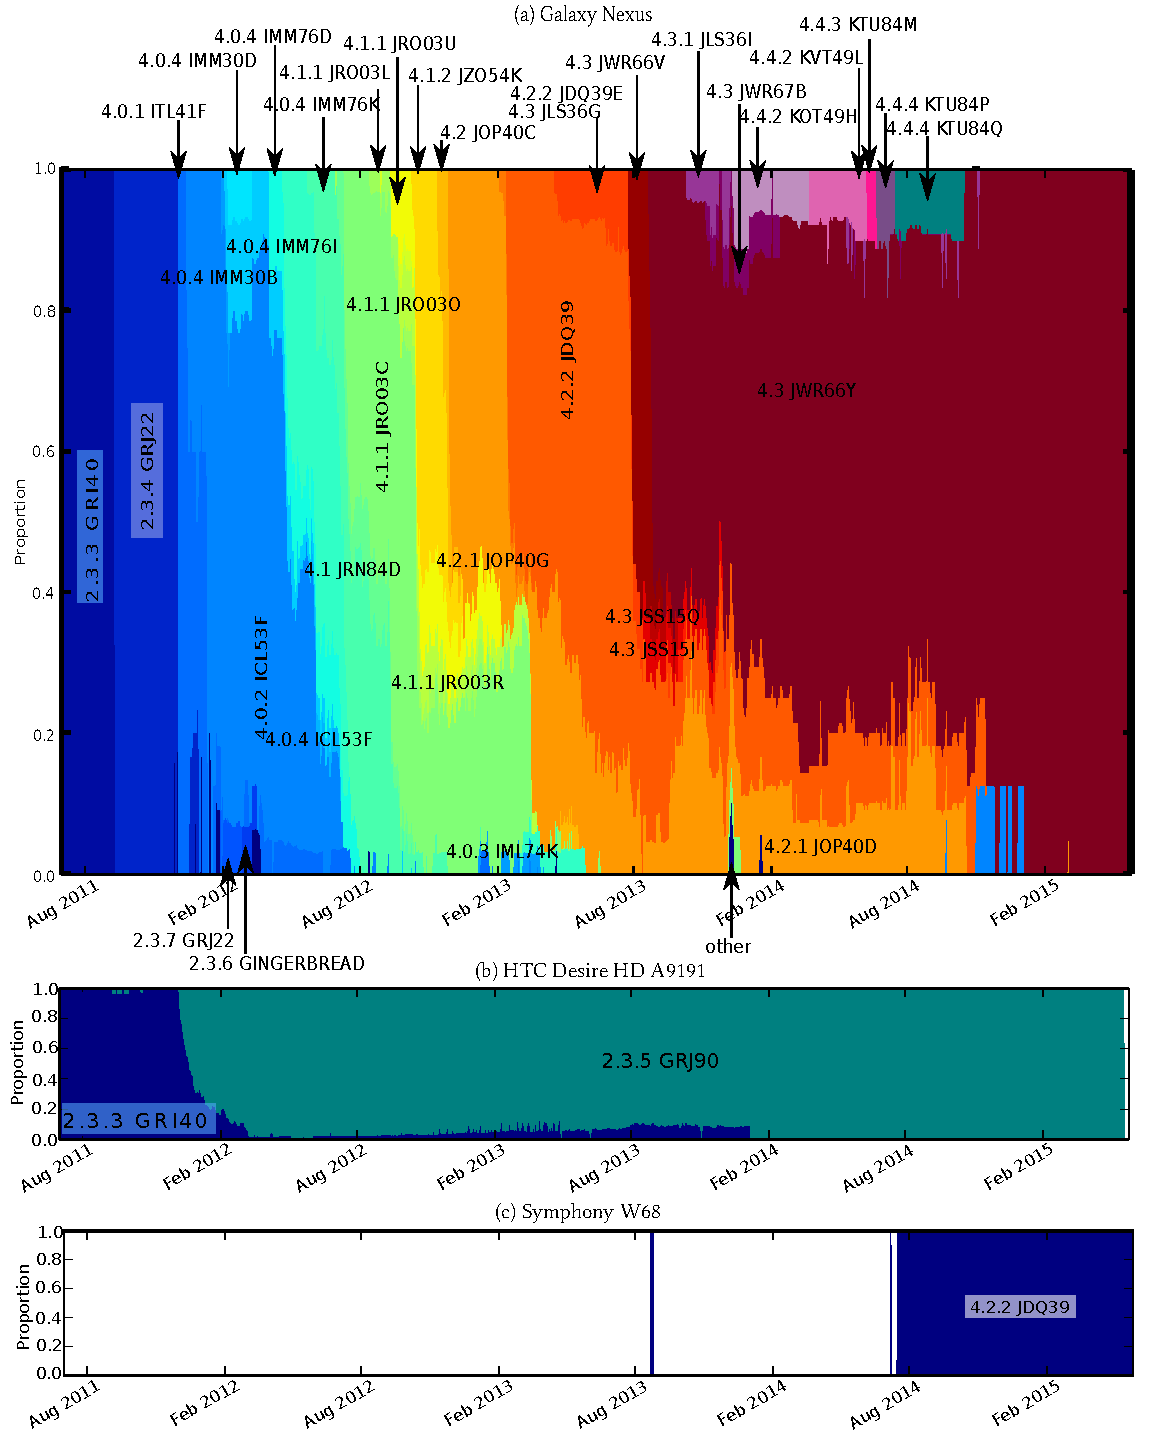
\includegraphics[width=0.9\textwidth]{figures/full_version_comp.pdf}
 \caption{Full version distributions for the highest and lowest scoring models}
 \label{fig:full_version_comp}
\end{figure*}

\daTabSecScoresoperator
We also analysed different network operators, for the \daNumSigOperators\ network operators with a significant presence in our data.
Table~\ref{tab:sec_operator} shows the results \emph{\daSecScoreBestoperator} (\daSecScoreBestoperatorScore\ out of 10) scoring highest and \emph{\daSecScoreWorstoperator} (\daSecScoreWorstoperatorScore\ out of 10) scoring lowest.
However the score of a network operator is affected by the device manufacturers of the devices which are in use on its network.
This is in turn affected by both what devices a network operator offers to users and upon which devices users choose.
Hence having a worse score does not necessarily mean that a network operator is worse, it could be that its users all pick phones from a worse device manufacturer, for example because they were cheaper.
A network operator could use data from this paper to exclude insecure devices from those offered to consumers.
An added value analysis of network operators which takes into account the device mix used by users of that network operator would make it possible to determine whether a network operator is making the situation better or worse by the way it ships updates to users.
However our sample size is too small to do that as while we have significant numbers of devices for each of the device models (Table~\ref{tab:sec_model}) and for each of the network operators (Table~\ref{tab:sec_operator}) we would need a significant number of each model in each network operator.
%We do not attempt to disambiguate users behaviour in whether they install updates from network operators using rolling upgrades.


\subsection{Scores over time}
\begin{figure}
\centering
\begin{subfigure}{\columnwidth}
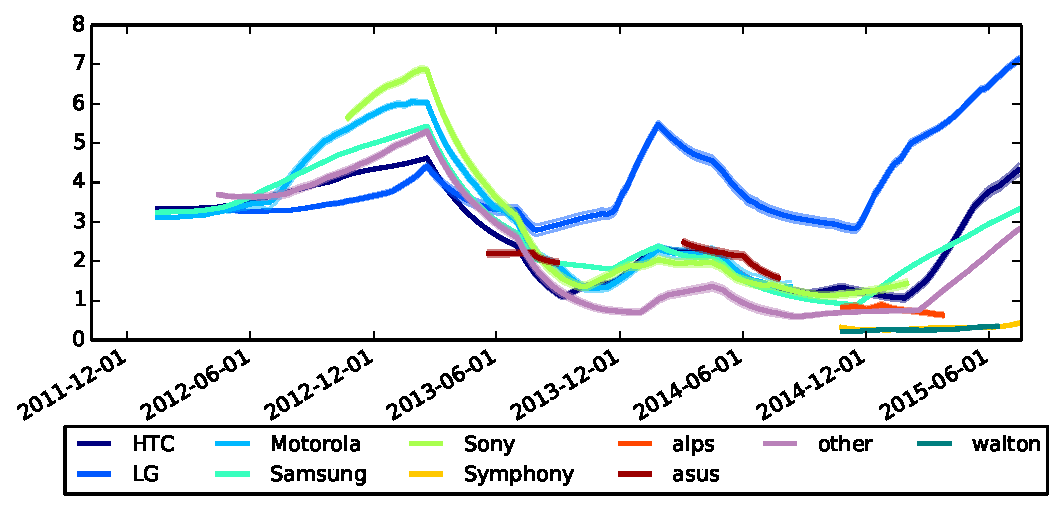
\includegraphics[width=\columnwidth]{figures/security_score_manufacturer}
\caption{Device manufacturers}
\label{fig:security_score_manufacturer}
\end{subfigure}
%
\begin{subfigure}{\columnwidth}
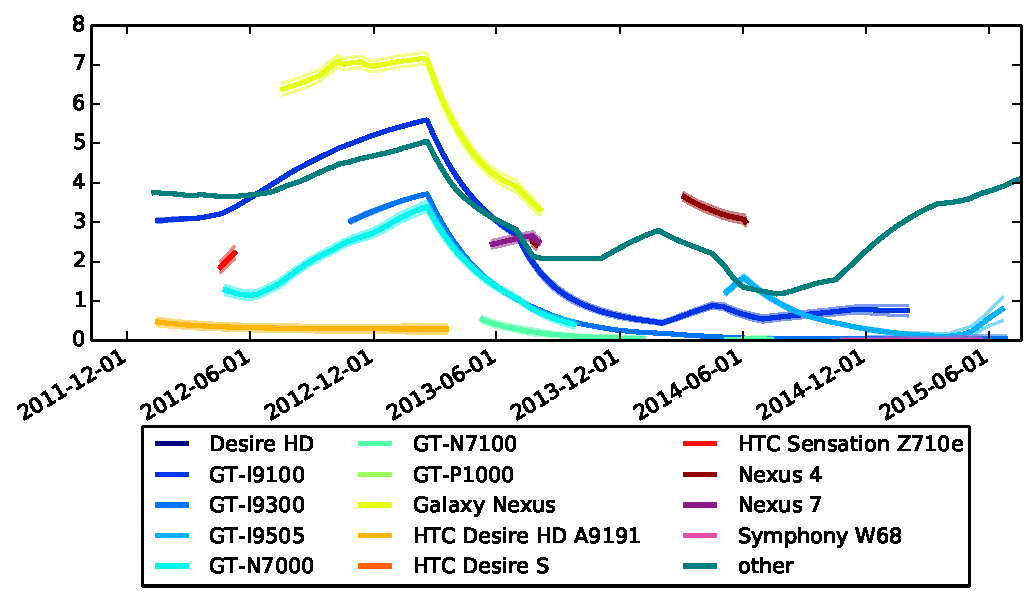
\includegraphics[width=\columnwidth]{figures/security_score_model}
\caption{Device models}
\label{fig:security_score_model}
\end{subfigure}
%
\begin{subfigure}{\columnwidth}
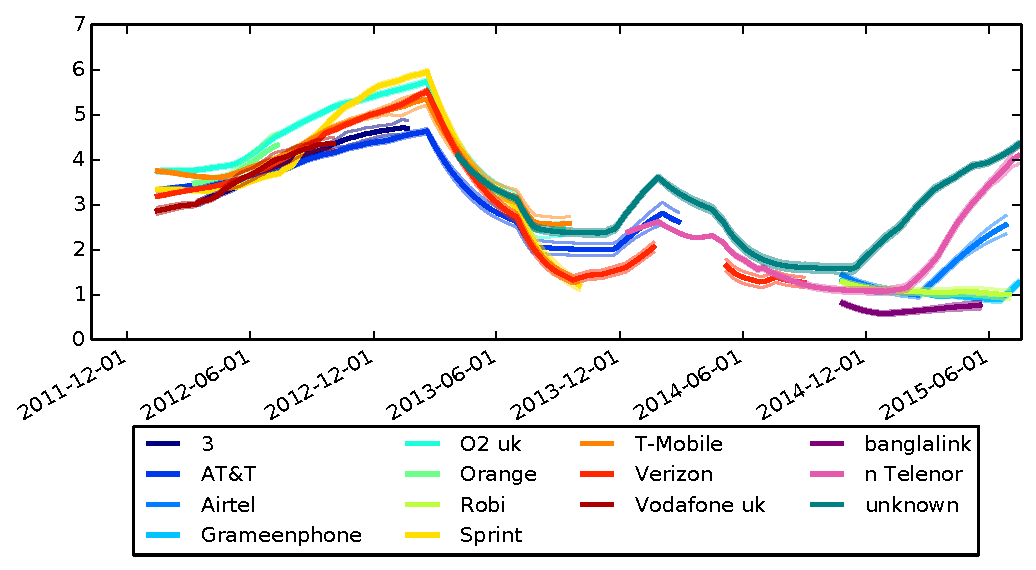
\includegraphics[width=\columnwidth]{figures/security_score_operator}
\caption{Network operators}
\label{fig:security_score_operator}
\end{subfigure}
%
\begin{subfigure}{\columnwidth}
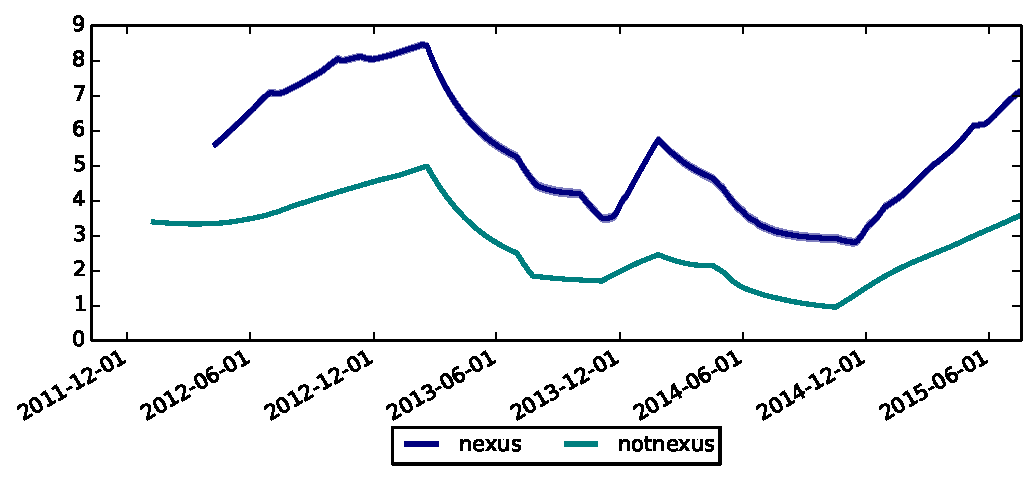
\includegraphics[width=\columnwidth]{figures/security_score_summary}
\caption{Nexus and non-Nexus devices}
\label{fig:security_score_summary}
\end{subfigure}
\caption{Security scores for device manufacturers, device models, network operators and Nexus devices. 95\% confidence intervals indicated.\todolater{bridge gaps?}}
\label{fig:security_scores}
\end{figure}
\todo{This is method rather than result}
The scoring metric as originally computed is averaged over the whole history of the device manufacturer, device model or network operator, it gives equal weight to periods years ago as to in the last few months.
If instead we take an exponential moving average of the daily score for days with more than \daSigNumDevicesDay\ devices when there have been at least consecutive \daSigNumDays\ days of data with that many devices then we can plot how this score has changed over time.
Equation~\ref{eq:rolling_update} shows how the value for a particular day ($v_i$) is computed from the previous day's value and the input for the current day ($n$) with an $\alpha$ of $1/\daSigNumDays$.
\begin{equation}
v_i = v_{i-1} (1 - \alpha) + n \alpha
\label{eq:rolling_update}
\end{equation}
Figure~\ref{fig:security_scores} shows this for manufacturers, device models, network operators and for Nexus and non-Nexus devices.
These show how the scores for different entities are different and change over time, while there is correlated behaviour for different entities (due to things like new vulnerabilities affecting all Android being discovered) these lines still have crossings due to the different behaviour of the different entities.
It also shows that we do not have sufficient data for all the entities all of the time, resulting in gaps in the data.
The clearest results are for Figure~\ref{fig:security_score_summary} with a large gap between the scores for Nexus and non-Nexus devices across the whole data set.


\subsection{Sensitivity of scoring metric}
\daTabDLDistances
\daTabChangeInScores
To evaluate whether the ranking of different manufacturers is sensitive to the form of the scoring metric we computed the normalised Damerau-Levenshtein distance~\cite{Bard2007} between the lists ordered using different forms of the scoring metric, this is shown in Table~\ref{tab:dl_distances}.
The `equal' metric weights $f$, $u$ and $m$ equally rather than favouring $f$ and makes little difference.
Changing the scoring metric also impacts the scores given for each entity Table~\ref{tab:change_in_scores} shows the mean impact on the scores.
This shows that $m$ tends to drag down scores.
\todo{Give some of the actual orderings as well for the most important ones}
\todo{Sensitivity of time based vs. global scores}

\subsection{Gaming the score}
If the comparative data given here is used to influence purchasing decisions then entities in the Android ecosystem might try to game the score rather than genuinely improve security.
$f$ is hard to game without doing a good job at security but it doesn't get any worse if there is already one known vulnerability and another is found.
A high value of $u$ could be achieved by only ever shipping one version but that would give low values for $f$ and $m$ (and not be attractive to new customers).
A high value of $m$ could be achieved by focusing on only one device at a time and ensuring that it gets updates but ignoring all others, but that would lower $f$ and $u$.%
One way to influence our scores would be to add additional devices to Device Analyzer which have good security, these would have to be real end user devices as we could detect fake ones, this would increase the size of our data set and would require providing genuinely good security to some users.
Therefore our score is secure against passive gaming attacks which changed the measured distribution but would require active defence against active gaming attacks which target the measurement devices.

\section{Comparison with other data}
Here we show that the \da\ data~\cite{Wagner2013} is representative for our purposes by comparing it with two other sources of data which provide an upper and lower bound on it.
The \da\ data is collected from devices across the world where users have voluntarily installed the app.
We have obtained comparable data on 5\,290 devices from a multinational FTSE 100 company's mobile device management database which includes company and employee owned devices, and from 5\,170\,000 matching User-Agent headers on all HTTP traffic for 30\% of Rwanda for a week.
\todo{citation for Rwanda dataset}
\begin{figure}
\centering
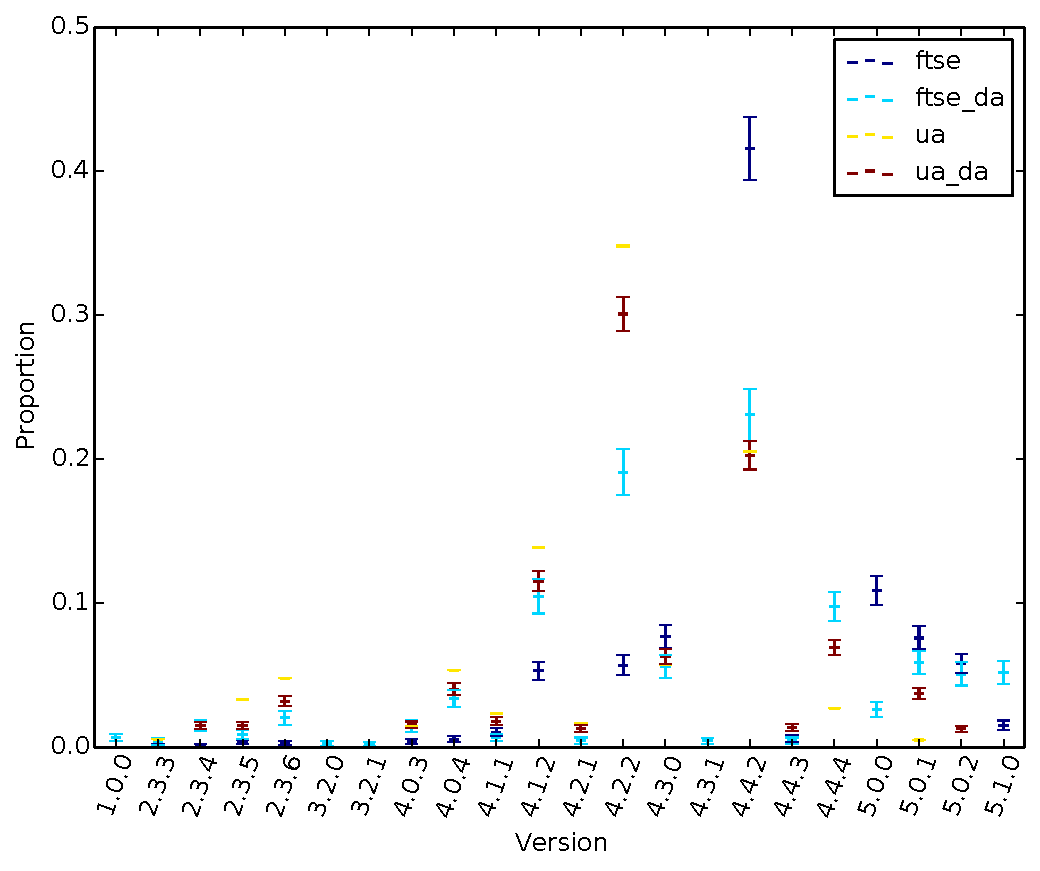
\includegraphics[width=\columnwidth]{figures/dists}
\caption{Comparison between FTSE, User-Agent and the corresponding \da\ data, error bars indicate 95\% confidence intervals.}
\label{fig:dists}
\end{figure}
We used the data from the FTSE 100 company for the week ending 2015-04-27 and the User-Agent data was collected between 2015-01-31 and 2015-02-12.
Figure~\ref{fig:dists} shows the proportion of devices running each Android OS version in the two comparison data sets and the comparable periods from \da.
The general pattern this shows is that in the FTSE data newer versions are more popular than in the \da\ data and that in the Rwanda data old versions are more popular than in the \da\ data.
\todo{Can we quantify this?}
This shows that \da\ lies between these two biased samples while being similar to both and so is representative.

\section{Related work}
The update process for apps, security fixes and OS upgrades also needs to be secure.
Unfortunately, package management systems designed to provide secure updates have been found to contain vulnerabilities~\cite{Cappos2008} and many software update systems fail to authenticate the connection between the device and the update server or do not authenticate the downloaded binaries~\cite{Bellissimo2006}.
Android does authenticate update binaries and Google Play downloads them over a secure connection~\cite{Viennot2014}.
In this paper we have analysed four critical vulnerabilities in the Android app update mechanism: APK unsigned shorts, APK unchecked name, APK duplicate file and Fake ID.
Other work has demonstrate complex and subtle errors exist in the Android app update process.
For example, the process can be exploited to allow apps to gain privilege through `Pileup' vulnerabilities by registering for new permissions before the update which creates that permission is installed~\cite{Xing2014}.

\interfootnotelinepenalty=10000 %To stop the lifehacker footnote below from spanning multiple pages and breaking
User-Agent strings have been used to investigate the timeliness of web browser updates, with at most 80\% of Firefox users running the most recent version~\cite{Frei2008}.
The same analysis was used to show that Chrome's use of silent updates seems to increase uptake of upgrades~\cite{Duebendorfer2010} with 97\% of users running the latest version within 3 weeks of release.
By way of comparison, Android's update process is manual.
The user is notified an update exists, but further action is required, including downloading the update and rebooting the phone to enable installation.
The phone must have sufficient charge to perform the update and the device itself is rendered inoperable during the update process, two factors which might prevent or delay the update process from taking place.
In our data we are unable to determine why a device is not updated. 
It is possible that many updates arrive at handsets, but are simply not installed.
Anecdotal evidence at least suggests that it is the lack of updates rather the lack of installation which is the major problem at present. Further work is required to tease these numbers apart.
Partly this is the result of the fact that an operating system update is being installed and so a reboot is required, but Chrome installs the new version side by side with the old one and switches the next time it is restarted.
The same technique would be more difficult on phones with limited storage space (as many cheap Android phones have barely enough space to install just the update) but is a plausible improvement for more high-end devices.
Google is deploying the same silent update technique through Google Play Services\footnote{\href{http://lifehacker.com/why-google-play-services-are-now-more-important-than-an-975970197}{http://lifehacker.com/why-google-play-services-are-now-more-important-than-an-975970197}} which automatically installs updates for core Google components of Android, this also bypasses the device manufacturer and network operator.

Security in depth is also a useful strategy.
In this regard, iOS provides additional safeguards beyond those used in Android, including a pre-distribution review, mandatory code-signing by the manufacturer, and (with the important exception of ROP-based attacks~\cite{Wang2013a}) the technical prohibition of dynamic code loading by an app.
These features, as well as Address Space Layout Randomisation (ASLR) and mandatory access controls, has resulted in a lower level of malware affecting iOS when compared to Android~\cite{Felt2011}.

There are continuing efforts to reduce the impact of critical vulnerabilities, both in Android and elsewhere.
SE\-Android~\cite{Smalley2013}, which is included in Android from version 4.1~\cite{jelly-bean-release}, and fully enforcing from version 5.0~\cite{AndroidSecurity2014} claimed to prevent some root vulnerabilities and to reduce the impact of others.
Capability based enforcement systems such as Capsicum~\cite{Watson2010} substantially reduce the capabilities that an exploit has to try and gain increased privilege with and could be included in Linux\footnote{\url{https://github.com/google/capsicum-linux}} and hence Android.

Rather than fixing critical vulnerabilities, security can be obtained by detecting malicious apps and preventing their installation or execution.
Detection strategies include Risk\-Ranker, which classified 3\,281 out of 118\,318 apps (2.8\%) as risky of which 718 (22\%) were malware and 322 (10\%) were previously unknown malware, an infection rate of 0.6\% across multiple markets~\cite{Grace2012a}.
Droid\-Ranger also analysed apps finding 148 out of 182\,823 apps (0.08\%) to be malicious across multiple markets of which 29 were previously unknown~\cite{Zhou2012a}.
%DroidRanger: It used permission-based behavioural fingerprinting which looked at the permissions of known malware and heuristic-based filtering -- dynamic loading of both Dalvik and native code.
A common technique used by attackers is to include malicious code in repackaged popular apps. 
An\-Darwin uses this insight to detect similar apps, and found 169 out of 265\,359 of all apps studied (0.06\%) were malicious clones~\cite{Crussell2013}.
%AnDarwin: It used clustering based on semantic vectors derived from the program dependence graphs to detect similar apps.

The percentage of Android devices running the most recent version (\daUpdatednessPerc) is much less than the rate ($>90$\%) for Windows XP SP2 computers contacting the Microsoft update servers~\cite{Gkantsidis2006}.
A simple numerical comparison is unfair because only one major OS version was considered in the Microsoft analysis, and data was only collected from computers which contacted the update server, although this was the default.
More recent data demonstrates the difficulty of upgrading computers between major OS versions, with 27\% of Windows computers running Windows XP in July 2014,\footnote{\url{https://archive.today/PLGxn}} four months after Windows XP stopped receiving security updates.

\cite{Nappa2015}
\cite{Zhang2014}
\cite{Lindorfer2014}
\cite{Arp2014}

\section{Conclusion}
 and examined how the Android ecosystem results in different device models receiving different levels of security due to whether or not they get security updates
We have compared different device models, device manufacturers and network operators and found that there are differences between them which the discerning purchaser might use to influence their decision about which device model to buy from which device manufacturer and network operator.
We hope that this analysis will encourage device manufacturers and network operators to improve the support they provide for devices after sale.


\section*{Acknowledgements}
\identifying{
This work was supported by a Google focussed research award and the EPSRC Standard Research Grant EP/P505445/1.
}
Some of the raw data and source code will be made available.

\sloppy
\printbibliography


\end{document}
